\documentclass[a4paper,12pt,twoside,dfinal,spanish]{book} 

\input{comment.sty}
\begin{comment}
%start the 81% scaling trick (comment out for full A4)
\addtolength{\oddsidemargin}{-0.2345679in} % magic number = 1 - 1/0.81
\addtolength{\evensidemargin}{-0.2345679in}% see documentation scale package
\addtolength{\topmargin}{-0.2345679in} % for explanation
\mag=810 % basic TeX command for 81% scaling
\usepackage[a4, center, nodriver]{crop}
%\usepackage[a4, center, frame]{crop}
%end of 81% scaling trick
\end{comment} 

\usepackage[spanish, es-tabla]{babel}
\usepackage[utf8]{inputenc}
\usepackage{amsfonts}
\usepackage{amssymb}
\usepackage{herab}
\usepackage{time}
\usepackage{rotating}
\usepackage{epsfig}
\usepackage{pifont}
\usepackage{verbatim}
\usepackage{pstricks}
\usepackage{multirow}
\usepackage{units}    
\usepackage{threeparttable}
\usepackage{mathrsfs}    
\usepackage[colorlinks,allcolors=blue]{hyperref}
% \usepackage{axodraw}
\usepackage{fancyhdr}
\usepackage{cite}
\usepackage{array}
\usepackage{graphicx}
\graphicspath{ {/home/gonza/git/Tesis/images/} }
\usepackage{graphics}

\newcolumntype{P}[1]{>{\centering\arraybackslash}p{#1}}
\usepackage[bf]{caption2}% Bold face for captions 

\pagestyle{fancy}
%----------------
\textheight22.6cm \textwidth16.0cm
%\textheight23.0cm \textwidth16.0cm
\newlength{\dinwidth}
\newlength{\dinmargin}
\newlength{\medwwidth}
\setlength{\dinwidth}{21.0cm}
\setlength{\headwidth}{\textwidth}
\setlength{\headheight}{18.0pt}
\columnsep1cm


\setlength{\dinmargin}{\dinwidth}
\addtolength{\dinmargin}{-\textwidth}
\setlength{\dinmargin}{0.5\dinmargin}
\oddsidemargin -1.0in
\setlength{\medwwidth}{-0.4cm}
\addtolength{\oddsidemargin}{\dinmargin}
\addtolength{\medwwidth}{\textwidth}
\setlength{\evensidemargin}{\oddsidemargin}
\setlength{\marginparwidth}{0.9\dinmargin}
\marginparsep 8pt \marginparpush 5pt
\topmargin0.0cm

%----------------------------------
\fancyhead{}
%\fancyhead[LE,RO]{\thepage}
%\fancyhead[LE]{\slshape {\bf \thepage}~~~~ \leftmark}
%\fancyhead[RO]{\slshape \rightmark ~~~~{\bf \thepage}}
\fancyhead[LE,RO]{\thepage}
\fancyhead[RE]{\slshape \leftmark }
\fancyhead[LO]{\slshape \rightmark}
\cfoot{}
%----------------------------------


%===================================
\renewcommand{\chaptermark}[1]{%
  \markboth{%   
    \thechapter~%
      \ #1}
  {}}
\renewcommand{\sectionmark}[1]{%
  \markright{%
    \thesection~%
      \ #1}
  {}}   
\renewcommand{\headrulewidth}{0.6pt}
%===================================






 

% \hyphenation{levens-duur}
% \hyphenation{hier-bij}
% \hyphenation{beslis-sing}
% \hyphenation{ex-pe-rim-ments}                         


%%%%%%%%%%%%%%%%%%%%%%%%%%%%%%%%%%%%%%%%%%%%%%%%%%%%%%%%%%%%%%%%
\begin{document}

%changed!
\newcommand{\Bee}{\ensuremath{{b}}}
\newcommand{\bjpsiX}{\ensuremath{ \Bee\to\jpsi X}}
\newcommand{\bjpsi}{\ensuremath{\Bee \to\jpsi}}
\newcommand{\bjpsill}{\ensuremath{\Bee \to\jpsi\to l^+l^-}}
\newcommand{\bjpsiee}{\ensuremath{\Bee \to\jpsi\to e^+e^-}}
\newcommand{\bjpsimm}{\ensuremath{\Bee \to\jpsi\to \mu^+\mu^-}}
\newcommand{\sigbbar}{\ensuremath{\sigma(\bbar)}}
\newcommand{\dsigbbar}{\ensuremath{\Delta\sigma(\bbar)}}
\newcommand{\bbar}{\ensuremath{\Bee\overline{\Bee}}}
\newcommand{\ccbar}{\ensuremath{c \overline{c}}}

\newcommand{\pntobbar}{\ensuremath{pN\to \bbar }}
%

%\newcommand{\ee}{\ensuremath{{\mathrm e}^+{\mathrm e}^-}}
\newcommand{\ee}{\ensuremath{e^+e^-}}
\newcommand{\mm}{\ensuremath{\mu^+\mu^-}}
\newcommand{\bn}{\ensuremath{{\mathrm B}^0}}
%\newcommand{\Bee}{\ensuremath{{\mathrm b}}}
\newcommand{\bnbar}{\ensuremath{\mathrm \overline{B}^0}}
\newcommand{\bnd}{\ensuremath{\mathrm B^0_d}}
\newcommand{\bndbar}{\ensuremath{\mathrm \overline{B}^0_d}}
\newcommand{\bns}{\ensuremath{\mathrm B^0_s}}
\newcommand{\bnsbar}{\ensuremath{\mathrm \overline{B}^0_s}}
\newcommand{\asym}{\ensuremath{frac{\Gamma_{B^0}(t)   - \Gamma_{\overline{B^0}}(t) }
                         {\Gamma_{B^0}(t)   + \Gamma_{\overline{B^0}}(t) } } }
\newcommand{\jpsi}{\ensuremath{J/\psi}}
\newcommand{\jpsiX}{\ensuremath{\mathrm \jpsi X}}
%\newcommand{\bjpsiX}{\ensuremath{\mathrm b\to\jpsi X}}
%\newcommand{\bjpsi}{\ensuremath{\mathrm b\to\jpsi}}
\newcommand{\jpsill}{\ensuremath{\mathrm \jpsi\to l^+l^-}}
\newcommand{\jpsiee}{\ensuremath{\mathrm \jpsi\to e^+e^-}}
\newcommand{\jpsimm}{\ensuremath{\mathrm \jpsi\to \mu^+\mu^-}}
%\newcommand{\bjpsill}{\ensuremath{\mathrm b\to\jpsi\to l^+l^-}}
%\newcommand{\bjpsiee}{\ensuremath{\mathrm b\to\jpsi\to e^+e^-}}
%\newcommand{\bjpsimm}{\ensuremath{\mathrm b\to\jpsi\to \mu^+\mu^-}}
\newcommand{\ks}{\ensuremath{{\mathrm  K}^{\mathrm 0}_{\mathrm s}}}
\newcommand{\K}{\ensuremath{{\mathrm  K}^+}}
%\newcommand{\bbar}{\ensuremath{\mathrm \B\overline{\Bee}}}
%\newcommand{\sigbbar}{\ensuremath{\sigma(\bbar)}}
\newcommand{\xf}{\ensuremath{x_{ F}}}
\newcommand{\pt}{\ensuremath{p_{ T}}}


\newcommand{\dm}{\ensuremath{\Delta m} }
\newcommand{\dmd}{\ensuremath{\Delta m_{\mathrm d}}}
\newcommand{\egev}{\ensuremath{\, \mathrm{GeV}}}
\newcommand{\mgev}{\ensuremath{\, \mathrm{GeV}/c^2}}
\newcommand{\pgev}{\ensuremath{\, \mathrm{GeV}/c}}
\newcommand{\emev}{\ensuremath{\, \mathrm{MeV}}}
\newcommand{\mmev}{\ensuremath{\, \mathrm{MeV}/c^2}}
\newcommand{\pmev}{\ensuremath{\, \mathrm{MeV}/c}}
\newcommand{\mum}{\ensuremath{\, \mu\mathrm m}}
\newcommand{\acp}{\ensuremath{a_{\mathrm CP}}}
\newcommand{\ccp}{\ensuremath{c_{\mathrm CP}}}
\newcommand{\ecp}{\ensuremath{\epsilon_{\mathrm B}} }

     
% Some useful abbrevations
% modified by U. Husemann
%
% Journals etc.
%
\newcommand{\ARNP}[3]      {Ann.\ Rev.\ Nuc.\ Part.\ Sci.~{\bf #1} (#2) #3}
\newcommand{\IEEE}[3]      {IEEE Trans.\ Nucl.\ Sci.~{\bf NS-#1} (#2) #3}
\newcommand{\NIM}[3]       {Nucl.\ Instr.\ Methods~{\bf A#1} (#2) #3}
\newcommand{\NPA}[3]       {Nucl.\ Phys.~{\bf A#1} (#2) #3}
\newcommand{\NPB}[3]       {Nucl.\ Phys.~{\bf B#1} (#2) #3}
\newcommand{\PLB}[3]       {Phys.\ Lett.~{\bf B#1} (#2) #3}
\newcommand{\PRC}[3]       {Phys.\ Rev.~{\bf C#1} (#2) #3}
\newcommand{\PRD}[3]       {Phys.\ Rev.~{\bf D#1} (#2) #3}
\newcommand{\PRL}[3]       {Phys.\ Rev.\ Lett.~{\bf #1} (#2) #3}
\newcommand{\SJNP}[3]      {Sov.~J.\ Nucl.\ Phys.~{\bf #1} (#2) #3}
\newcommand{\ZPC}[3]       {Z.~Phys.~{\bf C#1} (1#2) #3}
\newcommand{\EPJ}[3]       {Eur.\ Phys.\ J.~{\bf C#1} (#2) #3}
\newcommand{\CPC}[3]       {Comp.\ Phys.\ Comm.~{\bf #1} (#2) #3}
\newcommand{\journal}[4]   {#1~{\bf #2} (#3) #4}
%
% Abbreviations
%
\newcommand{\hb} {\mbox{\sffamily HERA \protect\rule[.5ex]{1.ex}{.11ex} B}\ }
\newcommand{\hbp}{\mbox{\sffamily HERA \protect\rule[.5ex]{1.ex}{.11ex} B}}
\newcommand{\ra} {\mbox{$\mskip 3mu \rightarrow \mskip 5mu$}}
\newcommand{\mt} {\mbox{$p_\mathrm{T}$}}
\newcommand{\ptp}{\mbox{$\mt > 1.5~{\mathrm{GeV}/c}$}}
\newcommand{\mct}{\mbox{$M>4.5~{\mathrm{GeV}/c^2}$}}
\newcommand{\hpt}{\mbox{high-\mt}}
\newcommand{\nl} { \hfill\break }
%\newcommand{\sb} { \thinspace }
\newcommand{\np} { \vfill\eject }
%\newcommand{\ni} {\noindent}
\newcommand{\vspitem}{\vspace{-2truemm}}
\newcommand{\bbbar}{\mbox{$b\bar{b}$}}
\newcommand{\plmi}{\mbox{$\pm$}}
\newcommand{\x}{\mbox{$\times$}}
\newcommand{\chsq}{\mbox{$\chi^2$}}
\newcommand{\ddu}{\mbox{\"u}}
\newcommand{\ddo}{\mbox{\"o}}
%\newcommand{\bbar}{\mbox{$bar{b}$}}


\newcommand{\al} {$\alpha$}
\newcommand{\be} {$\beta$}
\newcommand{\co} {$^{60}$Co}
\newcommand{\sr} {$^{90}$Sr}
\newcommand{\dc} {$^\circ$C}
\newcommand{\ga} {$\gamma$}
\newcommand{\dk} {$^\circ$K}
\newcommand{\ko} {k$\Omega\cdot$cm}
\newcommand{\etal} {{\it et~al.}}
\newcommand{\flnu} {cm$^{-2}$}
\newcommand{\flxu} {cm$^{-2}$s$^{-1}$}
\newcommand{\neff} {$N_{eff}$}
\newcommand{\tflu} {$3\cdot 10^{14}$/cm$^2$}
\newcommand{\stflux} {$3\cdot 10^{7}$~cm$^{-2}$s$^{-1}$}

\newcommand{\eff}{\ensuremath{\varepsilon}}
\newcommand{\effB}{\ensuremath{\eff_B^{\jpsi}}}
\newcommand{\effBz}{\ensuremath{\eff_B^{\Delta z}}}
\newcommand{\effBt}{\ensuremath{\eff_B^{\rm tot}}}
\newcommand{\effP}{\ensuremath{\eff_P^{\jpsi}}}
\newcommand{\effPt}{\ensuremath{\eff_P^{\rm tot}}}
\newcommand{\effR}{\ensuremath{\eff_R}}
\newcommand{\bbjX}{\ensuremath{\bbar\ra\jpsi ~X}}
\newcommand{\jll}{\ensuremath{\jpsi\ra\dilepton}}
\newcommand{\lum}{\ensuremath{{\cal L}}}
\newcommand{\Br}{\ensuremath{{\rm  Br}}}
\newcommand{\sigB}{\ensuremath{\sigma_B^A}}
\newcommand{\sigP}{\ensuremath{\sigma_P^A}}
\newcommand{\dsigB}{\ensuremath{\Delta\sigma_B^A}}
\newcommand{\dsigP}{\ensuremath{\Delta\sigma_P^A}}

\newcommand{\Dz}{\ensuremath{\Delta z}}
\newcommand{\dz}{\ensuremath{\delta z}}
% the following commands are in accordance with the Elementary Particle 
% Entity Notation (PEN) conventions



%
% (anti-) B mesons and their masses
\newcommand{\bm}   {B~meson}                                            % B meson
\newcommand{\PB}   {\mbox{\ensuremath{\mathrm{B}}}}                     % B meson 
\newcommand{\PBp}  {\mbox{\ensuremath{\mathrm{B}^+}}}                   % B+ meson
\newcommand{\PBm}  {\mbox{\ensuremath{\mathrm{B}^-}}}                   % B- meson     
\newcommand{\PMB}  {\mbox{\ensuremath{m_{\mathrm{B}}}}}                 % B mass
\newcommand{\PBz}  {\mbox{\ensuremath{\mathrm{B}^0}}}                   % B0
\newcommand{\PaBz} {\mbox{\ensuremath{\overline{\mathrm{B}^0}}}}        % B0-bar
\newcommand{\PMBz} {\mbox{\ensuremath{m_{\mathrm{B}^0}}}}               % B0 mass
\newcommand{\PBzd} {\mbox{\ensuremath{\mathrm{B}^0_{\mathrm{d}}}}}      % B0d 
\newcommand{\PMBzd}{\mbox{\ensuremath{m_{\mathrm{B}^0_{\mathrm{d}}}}}}  % B0d mass
\newcommand{\PaBzd}{\mbox{\ensuremath{\overline{\mathrm{B}^0_{\mathrm{d}}}}}} % B0d-bar
\newcommand{\PBzs} {\mbox{\ensuremath{\mathrm{B}^0_{\mathrm{s}}}}}      % B0s 
\newcommand{\PMBzs}{\mbox{\ensuremath{m_{\mathrm{B}^0_{\mathrm{s}}}}}}  % B0s mass
\newcommand{\PaBzs}{\mbox{\ensuremath{\overline{\mathrm{B}^0_{\mathrm{s}}}}}} % B0s-bar 

% D mesons
\newcommand{\PDz} {\mbox{\ensuremath{\mathrm{D^0}}}}                    % D0
\newcommand{\PDps}{\mbox{\ensuremath{\mathrm{D^+_s}}}}                  % D+s
\newcommand{\PDms}{\mbox{\ensuremath{\mathrm{D^-_s}}}}                  % D-s

% the typical final states
%\newcommand{\PJgy}{\mbox{\ensuremath{\mathrm{J}\mskip -2mu/\mskip -2mu\psi}}} % J/Psi
\newcommand{\PJgy}{\ensuremath{{\rm J}/\psi}}                                  % J/Psi 
\newcommand{\PKz} {\mbox{\ensuremath{\mathrm{K}^0}}}                    % K0
\newcommand{\PKp} {\mbox{\ensuremath{\mathrm{K}^+}}}                    % K+
\newcommand{\PKm} {\mbox{\ensuremath{\mathrm{K}^-}}}                    % K-
\newcommand{\PKpm}{\mbox{\ensuremath{\mathrm{K}^\pm}}}                  % K+-
\newcommand{\PKzS}{\mbox{\ensuremath{\mathrm{K^0_S}}}}                  % Ks
\newcommand{\PKzL}{\mbox{\ensuremath{\mathrm{K^0_L}}}}                  % Kl
\newcommand{\PKst}{\mbox{\ensuremath{\mathrm{K^*(892)}}}}               % K*
\newcommand{\dilepton}{\mbox{\ensuremath{\ell^+ \ell^-}}}               % lepton pair
\newcommand{\epem}{\mbox{\ensuremath{\mathrm{e}^+ \mathrm{e}^-}}}       % e+ e-
\newcommand{\mpmm}{\mbox{\ensuremath{\mu^+ \mu^-}}}                     % mu+ mu-
\newcommand{\pppm}{\mbox{\ensuremath{\pi^+ \pi^-}}}                     % pi+ pi-
\newcommand{\jpsiks}{\mbox{\ensuremath{\PJgy \mskip 5mu \PKzS}}}        % J/Psi Ks
\newcommand{\jmumu}{\mbox{\ensuremath{\jpsi \rightarrow \mu^+ \mu^-}}}   % J/Psi -> mu+ mu-



% some decays
%\newcommand{\bjpsi}{\mbox{$b \ra \jpsi$}}                               % b -> J/Psi
\newcommand{\btojpsi}{\mbox{$\PB \ra \jpsi$}}                           % B -> J/Psi
\newcommand{\bjp}{\mbox{$\PBz \ra \jpsiks$}}                            % B0 -> J/Psi Ks
\newcommand{\bsbs}{\mbox{$\PBzs - \PaBzs$}}                             % B0s - B0sbar
\newcommand{\bpp}{\mbox{$\PBz \ra \pppm$}}                              % B0 -> pu+ pi-
\newcommand{\bkp}{\mbox{$\PBz \ra \PKp \mskip 5mu \pi^-$}}              % B0 -> K+ pi-
\newcommand{\bpa}{\mbox{$\PBz \ra \pi^{\mp} \mskip 5mu a_1^{\pm}$}}     % B0 -> pi-+ a1+-
\newcommand{\bdk}{\mbox{$\PBp \ra \PDz \mskip 5mu \PKp$}}               % B+ -> D0 K+
\newcommand{\brk}{\mbox{$\PBp \ra \rho^0 \mskip 5mu \PKp$}}             % B+ -> rho0 K+
\newcommand{\bks}{\mbox{$\PBp \ra \pi^+ \mskip 5mu PKst$}}              % B+ -> pi+ K*
\newcommand{\brp}{\mbox{$\PBp \ra \pi^+ \mskip 5mu \rho^0$}}            % B+ -> pi+ rho0
\newcommand{\bsk}{\mbox{$\PBzs \ra \mathrm{D^{\mp}_s} \mskip 5mu \PKpm$}}% B0s -> D0s-+ K+-
\newcommand{\bsp}{\mbox{$\PBzs \ra \PDms \mskip 5mu \pi^+$}}            % B0s -> D-s pi+
\newcommand{\bsa}{\mbox{$\PBzs \ra \PDms \mskip 5mu 3\pi^{\pm}$}}       % B0s -> D-s 3 pi+-

\newcommand{\bjkp}{\mbox{$\PBz \ra \jpsi \mskip 5mu \PKp \mskip 5mu \pi^-$}}       % B0 -> J/Psi K+ pi-   
\newcommand{\bjk}{\mbox{$\PBp \ra \jpsi \mskip 5mu \PKp$}}              % B+ -> J/Psi K+    
%
% end
%%%%%%%%%%%%%%%%%%%%%%%%%%%%%%%%%%%%%%%%%%%%%%%%%%%%%%%%%%%%%%%%%%%%%%%%%%%%%%%








% 
\newgeometry{top=2cm,bottom=1.5cm,left=3cm,right=3cm}


\thispagestyle{empty}
\begin{center}

\begin{figure}[h]
\centering

\includegraphics[width=0.4\textwidth]{escudo}
\end{figure}

{\large Universidad Nacional de La Plata\\}
{\large Facultad de Ciencias Exactas\\}
{\large Departamento de Física\\}

% \hline

\vspace{2cm}

\hrulefill

{\bf \huge  Estudios de fondos de electrones reconstruidos como fotones en búsquedas de Supersimetría con el detector ATLAS\\}

\vspace{0.6cm}

\hrulefill

\vspace{0.3cm}

{\large \bf Trabajo de Diploma \\}

\vspace{2.5cm}

{\Large \bf Gonzalo E. Orellana \\}

\vspace{2.5cm}

{\Large\bf Director \\}
{\Large\bf Dr. Hernán P. Wahlberg \\}

\vspace{3cm}

{\large Marzo 2017}

\end{center}



\restoregeometry



 

\pagenumbering{roman}    

\tableofcontents  
   
\cleardoublepage 

\pagenumbering{arabic}

\setcounter{page}{1}

\pagestyle{fancy}

\chapter{Modelo Estándar y Supersimetría}
% \addcontentsline{toc}{chapter}{Modelo Estándar y Supersimetría}
\chaptermark{Modelo Estándar y Supersimetría}


El Modelo Estándar (SM, por sus siglas en inglés) es la teoría que describe a las partículas elementales y a sus interacciones. Este modelo fue introducido por Glashow, Salam y Weinberg en la década de los 70 \cite{Glashow:1961tr,Salam:1968rm,Weinberg:1967tq}. Está basado en teorías cuánticas de campo, y sus predicciones, cuantitativas y cualitativas, han sido verificadas experimentalmente con gran precisión.

Una de las extensiones del SM mejor motivada desde el punto de vista teórico es la Supersimetría, ya que resuelve algunas de las limitaciones del mismo. En particular, provee una solución al problema de jerarquía, proporciona candidatos para la materia oscura, permite la unificación de las fuerzas del SM, y hasta propone una conexión entre estas y la gravedad. Es por este motivo, que la Supersimetría, se ha vuelto uno de los objetivos principales en la búsqueda de nueva física en los últimos años.

\section{Modelo Estándar}
 
Según el SM las partículas se clasifican en dos grandes grupos: fermiones y bosones. Los fermiones son los que componen la materia ordinaria y se caracterizan por obedecer la estadística de Fermi-Dirac y tener espín semientero. Estos se clasifican en leptones y quarks, según si experimentan o no la interacción fuerte, siendo los últimos los que pueden interactuar mediante dicha fuerza.  

Existen 6 tipos (o sabores) de leptones que se clasifican en tres generaciones. Cada generación se forma a partir de un leptón masivo y cargado y otro no masivo y neutro. Así se tienen el electrón ($e^{-}$) con su correspondiente neutrino ($\nu_{e}$), y el muón ($\mu^{-}$) y el tau ($\tau^{-}$) con sus neutrinos asociados ($\nu_{\mu}$ y $\nu_{\tau}$ ).


Así mismo, existen 6 tipos de quarks: up ($u$), down ($d$), charm ($c$), strange ($s$), top ($t$) y bottom ($b$). A diferencia de los leptones, lo quarks tienen carga de color, que les permite interactuar mediante la fuerza fuerte. Los quarks solo se manifiestan en estados ligados, denominados hadrones, fenómeno conocido
como confinamiento de quarks. Existen dos tipos de hadrones en la naturaleza: los bariones ($qqq$) y los mesones ($q\bar{q}$).

Los fermiones se pueden encontrar en dos estados de helicidad, izquierda y derecha, salvo los neutrinos que solamente existen en estados de helicidad izquierda. Las dos últimas generaciones de fermiones son inestables, por lo que decaen a las de la primera generación. Es por esto que la materia ordinaria está compuesta por fermiones de la primera generación.

Así como los fermiones están asociados a la materia, los bosones están asociados a los portadores de las interacciones. Los mismos se caracterizan por obedecer la estadística Bose-Einstein y por tener espín entero. Existen cuatro tipos de interacciones fundamentales. La electromagnética, que afecta a las partículas con carga eléctrica, cuyo bosón asociado es el fotón. La débil, que actúa tanto en los quarks como en los leptones, asociada a los bosones $W^{\pm}$ y $Z^{0}$. La interacción fuerte, que actúa en las partículas con carga de color, cuyo portador son los gluones. Finalmente, la cuarta interacción es la gravitatoria. La misma no está descripta por el SM, pero supone que debería actuar sobre todas las partículas del SM y su bosón asociado sería el gravitón.

Todas las partículas anteriormente mencionadas, tienen asociadas una antipartícula con la misma masa y espín, pero con carga y varios de sus números cuánticos opuestos (isospín, charmness, strangeness, topness, número bariónico, etc.). 

El SM se construye formalmente como una teoría de gauge no abeliana, imponiendo invarianza de gauge local sobre campos cuantificados que describen las partículas fundamentales, dando lugar a los campos de gauge que describen las interacciones. Su grupo de simetría es:

\begin{equation}
\mathcal{G}_{SM}=SU(3)_{C}\times SU(2)_{L}\times U(1)_{Y}
\end{equation}

\noindent
donde $Y$ (la hipercarga), $L$ (la helicidad izquierda) y $C$ (la carga de color) representan las cantidades conservadas del grupo de simetría. El subgrupo $SU(2)_{L}\times U(1)_{Y}$ representa el sector electrodébil (QED + interacción débil) y el subgrupo $SU(3)_{C}$ incluye la cromodinámica cuántica (QCD).


En el SM las partículas adquieren su masa mediante el mecanismo de Brout-Englert-Higgs (BEH) \cite{Englert:1964et,Higgs:1964ia,Higgs:1964pj,Guralnik:1964eu,Higgs:1966ev,Kibble:1967sv} , a partir de la ruptura espontanea de la simetría electrodébil:

\begin{equation}
\mathcal{G}_{SM}\rightarrow SU(3)_{C}\times U(1)_{Q}
\end{equation}

\noindent
produciendo los bosones masivos $W^{\pm}$ y $Z^{0}$. Como consecuencia, es necesario incluir en el lagrangiano un nuevo campo escalar, dando lugar a un nuevo bosón masivo de espín 0, llamado bosón de Higgs. El mismo fue descubierto en el año 2012 por las colaboraciones ATLAS y CMS \cite{Aad:2012tfa, Chatrchyan:2012xdj}. La medida más reciente de su masa se determinó con un valor de $125.09 \pm 0.21 (\text{estad.}) \pm 0.11 (\text{sist.}) \egev$ \cite{Aad:2015zhl}. Así como los bosones de gauge adquieren su masa mediante este mecanismo, es posible también generar la masa de los fermiones mediante su interacción con el Higgs, completando de esta forma el espectro de masas del SM. La Tabla \ref{smparticles} expone algunas propiedades de las partículas mencionadas.

\renewcommand{\arraystretch}{1.3}
\begin{table}	
\centering
\caption{Partículas elementales del SM.}
\begin{tabular}{ l | c  c  c | c c }

	\hline

		& \multicolumn{3}{c}{Partículas} & Espín & Carga eléctrica \\

	\hline

	\multirow{3}{*}{Quarks} & $(u,d)_{L}$ & $(c,s)_{L}$ & $(t,b)_{L}$ & $(\frac{1}{2},\frac{1}{2})$ & $(\frac{2}{3},-\frac{1}{3})$ \\

							& $u_{R}$ & $c_{R}$ & $t_{R}$ & $\frac{1}{2}$ & $\frac{2}{3}$ \\

							& $d_{R}$ & $s_{R}$ & $b_{R}$ & $\frac{1}{2}$ & $-\frac{1}{3}$ \\

	\hline

	\multirow{2}{*}{Leptones} 	& $(\nu_{e},e^{-})_{L}$ & $(\nu_{\mu},\mu^{-})_{L}$ & $(\nu_{\tau},\tau^{-})_{L}$ & $(\frac{1}{2},\frac{1}{2})$ & $(0,-1)$ \\

								& $e_{R}^{-}$ & $\mu_{R}^{-}$ & $\tau_{R}^{-}$ & $\frac{1}{2}$ & $-1$ \\

	\hline

	\multirow{2}{*}{Bosones de Gauge} 	& \multicolumn{3}{c |}{$g$} & $1$ & $0$ \\

										& \multicolumn{3}{c |}{$W^{\pm}$, $Z$} & $1$ & $\pm1, 0$ \\

	\hline

	Bosones escalares & \multicolumn{3}{c |}{$H$} & 0 & 0 \\

	\hline

\end{tabular}
\label{smparticles}
\end{table}
\renewcommand{\arraystretch}{1}

Como comentario final, el SM tiene 19 parámetros libres: las 9 masas de los fermiones (considerando que los neutrinos tienen masa nula), las 3 constantes de acoplamiento de las interacciones, los 3 ángulos de mezcla de la matriz Cabibbo-Kobayashi-Maskawa (CKM) junto con la fase de la violación CP, el ángulo de vacío de QCD y finalmente la masa del Higgs y su valor de expectación del vacío.


\subsection{Física más allá del Modelo Estándar}

El SM provee una descripción notablemente exitosa de todos los fenómenos accesibles con los experimentos de altas energías disponibles actualmente. Sin embargo, también se sabe que el SM deja cuestiones sin resolver, tanto desde el punto de vista teórico, como experimental.

Desde el punto de vista teórico, el SM no explica los números cuánticos como la carga eléctrica, el isospín, la hipercarga o el color. Tampoco explica por qué los fermiones izquierdos se agrupan en dobletes y los derechos en singletes, ni por qué hay tres cargas de color, o cuántas generaciones hay. Otro síntoma de incompletitud es la gran cantidad de parámetros libres (19) que deben ajustarse a los datos observados, ya que no resultan de principios teóricos más fundamentales.

Desde el punto de vista experimental, también existen algunos resultados que no pueden acomodarse dentro del SM. Distintos experimentos demostraron que si bien los neutrinos tienen una masa muy pequeña, la misma no es nula. En contraposición con el SM que considera a los mismos no masivos. De todas formas, es posible escribir un término de masa para los neutrinos en el lagrangiano \cite{Drewes:2013gca}. El mismo requiere agregar parámetros adicionales a la teoría y además, de la existencia de neutrinos con quiralidad derecha, que aún no fueron observados.

El SM tampoco provee un candidato para la materia oscura. A partir de la observación del movimiento de las galaxias, se sabe que el mismo no se corresponde con la cantidad de materia observada, y es por eso que se propone la existencia de materia indetectable para los instrumentos astronómicos de medición actuales. La materia oscura debería corresponder entonces a partículas masivas, que interactúen solo débilmente y gravitacionalmente.

El triunfo de la teoría electrodébil, parece indicar que todas las interacciones corresponden a distintas manifestaciones de un único campo unificado y que el SM es una teoría efectiva a bajas energías (del orden de los $100\egev$). Incluso ante la ausencia de la gran unificación de las fuerzas electrodébil y fuerte a una escala muy alta de energía, el SM debería ser modificado para incorporar los efectos de la gravedad a la escala de Planck $M_{P} \simeq 10^{19} \egev$. En este contexto, es un misterio por qué la relación $M_{W}/M_{P} \simeq 10^{-17} \egev$ es tan pequeña, lo que se denomina <<problema de jerarquía>>\cite{PhysRevD.14.1667}. Esto lleva a pensar que los fenómenos de nueva física existen 17 órdenes de magnitud por arriba de la energía explorada en el presente. Asociado a este problema está el llamado <<problema de naturalidad>>, donde no se comprende por qué la masa del Higgs es tan pequeña comparada con masa de Planck.


\subsection{Divergencias cuadráticas}

Como se mencionó anteriormente, el SM ha tenido un gran éxito en la descripción de los fenómenos conocidos hasta la escala del TeV. Aun así, es clara la necesidad de construir una nueva teoría que solucione los problemas que el SM conlleva. El principal inconveniente es solucionar el <<problema de jerarquía>>, en el cual el cociente de escalas $M_{W}/M_{P}$ es muy pequeño. Para ello es necesario ver las consecuencias de esta diferencia de escalas.

La parte eléctricamente neutra del campo de Higgs del SM es un escalar complejo $H$ con un potencial clásico $V=m_{H}^{2}|H|^{2}+\lambda|H|^{4}$. El SM necesita un valor de expectación de vacío (VEV) para $H$ no nulo, en el mínimo del potencial. Esto ocurre si $\lambda >0$ y $m_{H}^{2}<0$, resultando en $\left\langle H \right\rangle = \sqrt{-m_{H}^{2}/2\lambda}$. Experimentalmente, de las medidas de las propiedades de las interacciones débiles, se sabe que el valor de $\left\langle H \right\rangle$ es de aproximadamente 174 GeV. El descubrimiento del bosón de Higgs en el 2012 con una masa cercana a 125 GeV implica que, suponiendo que el SM es correcto como una teoría efectiva, $\lambda = 0.126$ y $m_{H}^{2}=-(92.9\: \egev)^{2}$.

Por cada partícula a la que se acopla el campo de Higgs, $m_{H}^{2}$ recibe una gran corrección cuántica de los efectos virtuales. Por ejemplo, si el campo de Higgs se acopla a un fermión $f$ con un término en el lagrangiano igual a $-\lambda H\bar{f}f$, el diagrama de Feynman en la Figura \ref{loops} genera una corrección:

\begin{equation}
\Delta m_{H}^{2}=-\frac{|\lambda_{f}|^{2}}{8\pi^{2}}\Lambda_{UV}^{2}+...
\label{fermion_corr}
\end{equation}

\noindent
donde $m_{f}$ es la masa del fermión y $\Lambda_{UV}$ es el corte usado para regular la integral en el loop. 

\begin{figure}
\centering

	\begin{subfigure}{0.45\textwidth}
	\begin{tikzpicture}
	\begin{feynman}
	\vertex (a) {\(H\)};
	\vertex [right=2cm of a] (b);
	\vertex [above right=of b] (e);
	\vertex [below right=of b] (f);
	\vertex [above right=of f] (c);
	\vertex [right=2cm of c] (d);
	\diagram* {
	(a)-- [scalar] (b),
	(b)-- [fermion, quarter left, edge label=\(f\)] (e),
	(e)-- [quarter left] (c),
	(c)-- [quarter left, fermion] (f),
	(f)-- [quarter left] (b),
	(c)-- [scalar] (d),
	};
	\end{feynman}
	\end{tikzpicture}
	\end{subfigure}
	\hfill
	\begin{subfigure}{0.45\textwidth}
	\begin{tikzpicture}
	\begin{feynman}
	\vertex (a) {\(H\)};
	\vertex [right=3cm of a] (b);
	\vertex [above left=of b] (d);
	\vertex [above right=of b] (f);
	\vertex [above right=of d] (e);
	\vertex [right=3cm of b] (c);
	\diagram* {
	(a)-- [scalar] (b),
	(b)-- [scalar, quarter left] (d),
	(d)-- [quarter left, scalar, edge label=\(S\)] (e),
	(e)-- [quarter left, scalar] (f),
	(f)-- [quarter left, scalar] (b),
	(b)-- [scalar] (c),
	};
	\end{feynman}
	\end{tikzpicture}
	\end{subfigure}

\caption{Correcciones cuánticas a un \textit{loop} al parámetro de masa del Higgs $m_{H}^{2}$ debido a la masa de un fermión de Dirac \textit{f} (izquierda) y debido a la masa de un campo escalar \textit{S} (derecha).}
\label{loops}
\end{figure}

Si $\Lambda_{UV}$ es del orden de $M_{P}$, la corrección a $m_{H}^{2}$ es 30 órdenes de magnitud más grande que el valor requerido $\sim (100\: \egev)^{2}$, produciendo las divergencias cuadráticas. Si bien los fermiones y bosones de gauge no tienen este comportamiento cuadrático en las correcciones cuánticas (sus masas son “naturales”), también se ven afectados indirectamente por este efecto, ya que las masas de los mismos dependen de $\left\langle H \right\rangle$. De esta forma, todas las masas de SM se ven afectadas por la escala de corte $\Lambda_{UV}$.

Una forma de solucionar este problema consiste en considerar la existencia de un escalar complejo $S$ de masa $m_{S}$, que se acopla al campo de Higgs con un término $-\lambda_{S} |H|^{2}|S|^{2}$. El diagrama de Feynman de la Figura \ref{loops} genera una corrección:

\begin{equation}
\Delta m_{H}^{2}=\frac{\lambda_{S}^{2}}{16\pi^{2}}\left[\Lambda_{UV}^{2}-2m_{S}^{2}\ln(\Lambda_{UV}^{2}/m_{S})+... \:\right]
\label{boson_corr}
\end{equation}

% \begin{figure}
% \centering
% \begin{tikzpicture}
% \begin{feynman}
% \vertex (a) {\(H\)};
% \vertex [right=3cm of a] (b);
% \vertex [above left=of b] (d);
% \vertex [above right=of b] (f);
% \vertex [above right=of d] (e);
% \vertex [right=3cm of b] (c);
% \diagram* {
% (a)-- [scalar] (b),
% (b)-- [scalar, quarter left] (d),
% (d)-- [quarter left, scalar, edge label=\(S\)] (e),
% (e)-- [quarter left, scalar] (f),
% (f)-- [quarter left, scalar] (b),
% (b)-- [scalar] (c),
% };
% \end{feynman}
% \end{tikzpicture}
% \caption{Correcciones cuánticas a un \textit{loop} al parámetro de masa del Higgs $m_{H}^{2}$ debido a la masa de un campo escalar \textit{S}.}
% \label{loop_f}
% \end{figure}

De esta forma, si existieran fermiones (bosones) no predichos por el SM, relacionados con los bosones (fermiones) del SM mediante una simetría, las contribuciones a las masas de las Ecuaciones \ref{fermion_corr} y \ref{boson_corr} se cancelarían. A esta simetría se la denomina supersimetría (SUSY, por sus siglas en inglés) \cite{Martin:1997ns}.


\section{Extensión Supersimétrica del Modelo Estándar}

Supersimetría es una simetría que relaciona las masas y los acoplamientos de partículas con diferente espín. Una transformación supersimétrica convierte un estado bosónico en uno fermiónico, y viceversa. El operador $Q$ que genera estas transformaciones debe ser un espinor anticonmutativo, que cumpla:

\begin{equation}
\centering
Q \ket{\text{\,bosón\,}} = \ket{\text{\,fermión\,}}
\qquad\qquad\qquad
Q \ket{\text{\,fermión\,}} = \ket{\text{\,bosón\,}}
\end{equation}

Los espinores son intrínsecamente objetos complejos, por lo tanto el conjugado hermítico de $Q$ es también un generador de la simetría. Debido a que $Q$ y $Q^{\dagger}$ son operadores fermiónicos, llevan momento angular de espín $\frac{1}{2}$, por lo tanto es claro que SUSY debe ser una simetría espacio-temporal.

Los estados de partícula de una teoría supersimétrica son representados en el álgebra de SUSY como supermultipletes. Cada supermultiplete contiene ambos estados, fermión y bosón, que son comúnmente llamados supercompañeros uno de otro. Los generadores $Q$ y $Q^{\dagger}$ conmutan con los generadores de las transformaciones de gauge, por lo tanto las partículas en un mismo supermultiplete tienen que estar en la misma representación del grupo de gauge, y tener la misma carga eléctrica, isospín y color. Y como el operador de masa $-P^{2}$ también conmuta con los generadores y con todos los operadores de rotación y traslación, deberán tener los mismos autovalores de $-P^{2}$ , y entonces la misma masa.

Cada supermultiplete tiene que contener igual número de grados de libertad fermiónico que bosónico ($n_{F}=n_{B}$), por lo que existen varias combinaciones posibles. Las dos más importantes para esta teoría son el supermultiplete quiral (o escalar) y el de gauge (o vectorial).

% El supermultiplete escalar tiene un único fermión de Weyl ($n_{F}=2$) y dos escalares reales ($n_{B}=1$). Estos dos escalares se suelen poner como un único campo escalar complejo.

% El supermultplete vectorial contiene un bosón vectorial de spin $1$. Para que la teoría sea renormalizable, tiene que ser un bosón de gauge no masivo, al menos antes de que la simetría de gauge sea espontáneamente rota. En este caso, este bosón contiene dos estados de helicidad ($n_{B}=2$). Por lo tanto su supercompañero es un fermión de Weyl de espín $\frac{1}{2}$, con dos estados de helicidad ($n_{F}=2$). Si en vez de esto, se intenta usar un fermión de espín $\frac{3}{2}$ la teoría no sería renormalizable. Los bosones de gauge deben transformar como la representación adjunta del grupo de gauge, por lo que sus compañeros fermiónicos, llamados <<gauginos>>, también.En el caso de incluir la gravedad, el gravitón de espín 2 (con dos estados de helicidad, n B = 2) tiene un supercompañero de espín llamado <<gravitino>>.

La inclusión de la Supersimetría resuelve varios de los problemas antes mencionados. La simetría cancela las divergencias cuadráticas en la corrección de la masa del Higgs. La corrección de términos de mayor orden requieren que la masa de la partícula supersimétrica más liviana (\textit{Lightest Supersymmetric Particle}, LSP) sea del orden del TeV, siendo ese el orden de energía en el cual el SM deja de ser válido, y es necesaria la implementación de SUSY. También provee un candidato a materia oscura, siendo en la mayoría de los modelos la partícula supersimétrica más liviana, que es estable y no interactuante. Finalmente, SUSY provee un marco de referencia para una teoría de Gran Unificación y para teorías que incorporan a la gravedad. 



\subsection{Modelo Estándar Supersimétrico Mínimo}

Como se mencionó antes, en una extensión supersimétrica del SM, cada una de las partículas elementales conocidas está contenida en un supermultiplete quiral o de gauge, y debe tener un supercompañero con espín que difiera en $\frac{1}{2}$. La extensión que requiere la introducción de la mínima cantidad de parámetros se conoce como <<Modelo Estándar Supersimétrico Mínimo>> (MSSM por sus siglas en inglés).

Veamos ahora como se van construyendo los distintos supermultipletes. Como los supermultipletes escalares son los únicos que pueden contener un fermión cuya parte izquierda y derecha transforman de forma diferente, todos los fermiones del SM están agrupados en este tipo de supermultiplete. En cuanto a su nomenclatura, los nombres de los compañeros de espín 0 de los quarks o leptones son construidos anteponiendo una “s” (de scalar ), y son llamados <<squarks>> y <<sleptones>>. La parte izquierda y derecha de los quarks y leptones son fermiones de Weyl con diferentes propiedades de transformación de gauge del SM, entonces cada uno debe tener un compañero escalar complejo. Por ejemplo, los supercompañeros de la parte izquierda y derecha del campo de Dirac de los electrones son llamadas $\tilde{e}_{L}$ y $\tilde{e}_{R}$ , aunque el subíndice no se refiere a la helicidad de los slectrones (ya que ambos tienen espín 0) sino a la de sus supercompañeros. Lo mismo aplica para las demás leptones y quarks, los neutrino son simplemente denominados $\tilde{\nu}$ ya que son siempre izquierdos.

El bosón escalar de Higgs debe estar en un supermultiplete quiral ya que tiene espín 0. Dada la naturaleza de los campos quirales introducidos en la implementación de SUSY, el campo escalar de Higgs no es suficiente para dar masa a los fermiones de helicidad izquierda y derecha, por lo que se debe agregar un nuevo campo escalar para compensar. En el SM, el campo de Higgs es un doblete, y de los cuatro grados de libertad solo uno permanece como consecuencia de la ruptura de la simetría electrodébil, resultando en un bosón de Higgs. En el MSSM se necesitan dos dobletes de Higgs, $H_{u}=(H^{+}_{u},H^{0}_{u})$ y $H_{d}=(H^{0}_{d},H^{-}_{d})$. El escalar neutro que corresponde al bosón de Higgs del SM es una combinación lineal de $H^{0}_{u}$ y $H^{0}_{d}$. La nomenclatura usual para referirse a los supercompañeros de espín  es agregar “-ino” a la partícula del SM, por lo tanto los compañeros fermiónicos de los escalares de Higgs son denominados <<higgsinos>>, y se denotan $\widetilde{H_{u}}$ y $\widetilde{H_{d}}$.

Los bosones vectoriales del SM tienen que estar en supermultipletes de gauge y sus supercompañeros fermiónicos son llamados <<gauginos>>. Las interacciones de gauge de color de QCD son mediadas por el gluon, cuyo compañero supersimétrico de espín  es el <<gluino>>. Los gauginos supercompañeros de los bosones de gauge electrodébiles, luego de mezclarse con los supercompañeros de los bosones de Higgs, dan lugar a los autoestados de masa denominados <<charginos>> y <<neutralinos>>. En la Tabla \ref{susyparticles} se puede ver el espectro completo del MSSM.


\renewcommand{\arraystretch}{1.3}
\begin{table}	
\centering
\begin{threeparttable}
\caption{Supermultipletes quirales y de \textit{gauge} del MSSM.}
\begin{tabular}{ P{4cm} P{4cm} P{4cm} }

	\hline

	Supermultiplete & Bosón & Fermión \\

	\hline

	gluón, gluino & $g$ & $\widetilde{g}$ \\

	\hline

	W, wino & $W^{\pm}$, $W^{0}$ & $\widetilde{W}^{\pm}$, $\widetilde{W}^{0}$ \\
	B, bino & B & $\widetilde{B}$ \\

	\hline

	\multirow{2}{*}{sleptón, leptón $^{*}$} 	& $(\widetilde{\nu},\widetilde{e})_{L}$ & $(\nu,e)_{L}$ \\

										& $e_{R}$ & $e_{R}$ \\

	\hline

	\multirow{3}{*}{squark, quark $^{*}$}		& $(\widetilde{u}_{L},\widetilde{d}_{L})$ & $(u_{L},d_{L})$ \\

										& $\widetilde{u}_{R}$ & $u_{R}$ \\

										& $\widetilde{d}_{R}$ & $d_{R}$ \\

	\hline

	\multirow{2}{*}{Higgs, higgsinos}	& $(H^{0}_{d},H^{-}_{d})$ & $(\widetilde{H}^{0}_{d},\widetilde{H}^{-}_{d})$ \\

										& $(H^{+}_{u},H^{0}_{u})$ & $(\widetilde{H}^{+}_{u},\widetilde{H}^{0}_{u})$ \\

	\hline
\end{tabular}
\begin{tablenotes}
\item [*] \footnotesize Junto con las otras dos generaciones.
\end{tablenotes}
\label{susyparticles}
\end{threeparttable}
\end{table}
\renewcommand{\arraystretch}{1}


Por construcción, cada partículas y su supercompañero debe tener la misma masa, por lo que deberían existir, por ejemplo, fotinos de masa nula y selectrones con $0.511 \emev$. Como ninguna de las partículas antes mencionada fue observada experimentalmente, se deduce que SUSY es una simetría que está rota en el estado de vacío elegido por la naturaleza.

El hecho de que sea una simetría rota, impide que se cancelen las divergencias cuadráticas en el cuadrado de las masas escalares, y eso fue uno de los motivos por el cual se introdujo SUSY. Para poder garantizar que siga ocurriendo esa cancelación, la ruptura de la simetría debe ser suave, y el lagrangiano efectivo del MSSM tiene que escribirse como:

\begin{equation}
\mathcal{L}=\mathcal{L}_{\text{SUSY}}+\mathcal{L}_{\text{soft}}
\end{equation}

\noindent
donde $\mathcal{L}_{\text{SUSY}}$ contiene todas las interacciones de gauge y de Yukawa, y preserva la invarianza supersimétrica. 
% El conjunto de parámetros que aparecen en el lagrangiano $\mathcal{L}_{SUSY}$ son:

% \begin{itemize}

% 	\item las constantes de acoplamiento de gauge $g_{s}$, $g$ y $g'$ correspondientes a los grupos de gauge $SU(3)_{C}$, $SU(2)_{L}$ y $U(1)_{Y}$, respectivamente

% 	\item los acoplamientos de Yukawa que describen las interacciones entre fermiones y bosones de Higgs

% 	\item el parámetro de masa del campo de Higgs $\mu$.

% \end{itemize}


El lagrangiano que rompe SUSY, $\mathcal{L}_{\text{soft}}$, no está completamente determinado y su forma explícita así como el conjunto de parámetros involucrados dependen del mecanismo particular de ruptura de SUSY. Debido a que este mecanismo es desconocido, se puede suponer un conjunto de términos de ruptura de la forma más general posible, sin indagar en sus orígenes, que se fijan solo pidiendo la invarianza frente $SU(3)_{C}\times SU(2)_{L}\times U(1)_{Y}$, y que sean suaves a fin de mantener la cancelación de las divergencias cuadráticas. Estos términos soft proveen exitosamente las masas de las partículas supersimétricas, a fin de que sean más pesadas que sus correspondientes compañeras del SM, y la ruptura espontánea de la simetría electrodébil requerida a bajas energías necesaria para explicar la generación de las masas de las partículas del SM. Aun así, la diferencia de masa entre supercompañeros no debe ser demasiado grande, ya que se perdería la solución al problema de jerarquía.

% El conjunto de nuevos parámetros que aparece en el superpotencial de ruptura de SUSY incluye \cite{Agashe:2014kda,Haber:1993wf}:

% \begin{itemize}
 
% 	\item Las masas soft del sector de Higgs, $m_{1}$ , $m_{2}$ y $m_{12}$ , donde $m_{12}^{2} \equiv B\mu$, $\mu$ es el parámetro introducido anteriormente y $B$ es el parámetro de ruptura de SUSY.

% 	\item Las masas soft de los squarks y sleptones de cada generación: $m_{\tilde{Q}}$ , $m_{\tilde{U}}$ , $m_{\tilde{D}}$ , $m_{\tilde{L}}$ y $m_{\tilde{E}}$ .

% 	\item Los acoplamientos trilineales de squarks y sleptones $A_{q}$ y $A_{l}$.

% 	\item Las masas soft de los gauginos, $M_{3}$ , $M_{2}$ y $M_{1}$ , asociadas a los grupos de gauge del $SU(3)_{C}$, $SU(2)_{L}$ y $U(1)_{Y}$, respectivamente.

% \end{itemize}

Adicionalmente, para evitar problemas con la conservación del número bariónico $B$ y leptónico $L$, se introduce una nueva simetría denominada paridad-R. Se define como $P_{R}=(-1)^{3(B-L)+2s}$, donde $s$ es el espín de la partícula. Las partículas supersimétricas tienen $P_{R}=-1$, mientras que las partículas del SM tienen $P_{R}=+1$. La conservación de la paridad-R genera que las partículas supersimétricas solo puedan ser producidas en número par en experimentos de colisiones.

El trabajo de la referencia \cite{Dimopoulos:1995ju} muestra que el MSSM posee 124 parámetros independientes. De estos, 18 corresponden a los parámetros del SM, uno corresponde al sector de Higgs (el análogo a la masa del Higgs del SM), y 105 son nuevos parámetros del modelo. 

Existen distintas propuestas para los mecanismos de ruptura de supersimetría. En la búsqueda asociada al presente trabajo, el modelado de la señal de SUSY se da en el contexto del modelo “Generalised Model of Gauge-Mediated Supersymmetry Breaking” (GGMSB). En este modelo, la supersimetría es rota en la escala del TeV en un sector oculto de estados inaccesibles por procesos del SM, y es propagada al sector visible del MSSM vía interacciones de bosones de gauge del grupo $SU(3)_{C} \times SU(2)_{L} \times U(1)_{Y}$ y gauginos.

En estos modelos con mediaciones de gauge, el gravitino es la partícula supersimétrica más ligera (LSP), con masas del orden del keV, estable y no interactuante, produciendo así energía faltante en la reconstrucción del evento en su estado final.

\subsection{El espectro de masas}

Los supercompañeros de las partículas del SM no son necesariamente los estados de masa del MSSM. Incluyendo efectos de ruptura de simetría electrodébil y supersimetría se producen estados de masa como mezcla de gauginos y higgsinos. La única excepción es el gluino que es un octeto de color y no se mezcla con otras partículas.

Las masas y mezclas de las distintas partículas tienen un rol importante en cuanto a su fenomenología y su correspondiente búsqueda experimental, por lo que se describen brevemente a continuación.


\subsubsection{El sector de Higgs} 

El escalar de Higgs en el MSSM consiste en dos dobletes del $SU(2)_{L}$ complejos, $H_{u}$ y $H_{d}$, con ocho grados de libertad reales. Luego de la ruptura de simetría electrodébil, tres de ellos son los bosones de Nambu-Goldstone, que corresponden a los modos longitudinales de los bosones masivos $Z$ y $W^{\pm}$. Los restantes cinco grados de libertad producen el bosón de Higgs físico del modelo. La siguiente nomenclatura es utilizada:
\begin{align*}
  H^{\pm} & : \text{par de bosones de Higgs cargados} \\
  A^{0} & : \text{bosón de Higgs neutral CP-impar} \\
  H^{0},\: h^{0} & : \text{bosones de Higgs neutrales CP-par} 
\end{align*}

Una de las predicciones bastantes sólidas de supersimetría es que debe haber al menos un bosón de Higgs liviano.


\subsubsection{Neutralinos y charginos}

Los higgsinos y los gauginos electrodébiles pueden combinarse debido a los efectos de la ruptura de simetría electrodébil. Los higgsinos neutros ($\widetilde{H}^{0}_{u}$ y $\widetilde{H}^{0}_{d}$) y los gauginos neutros ($\widetilde{B}$ y $\widetilde{W}^{0}$) se combinan para formar cuatro autoestados de masa llamados <<neutralinos>>, denotados $\widetilde{\chi}^{0}_{1}$, $\widetilde{\chi}^{0}_{2}$, $\widetilde{\chi}^{0}_{3}$ y $\widetilde{\chi}^{0}_{4}$, ordenados de forma ascendente por sus masas. El neutralino más liviano, $\widetilde{\chi}^{0}_{1}$, generalmente se considera como la LSP, ya que es una de las partículas del MSSM que puede ser un buen candidato para la materia oscura. 

Los higgsinos cargados ($\widetilde{H}^{+}_{u}$ y $\widetilde{H}^{-}_{d}$) y los winos ($\widetilde{W}^{+}$ y $\widetilde{W}^{-}$) se combinan para formar dos autoestados de masa con carga $\pm1$, denominados <<charginos>> y se denotan $\widetilde{\chi}^{\pm}_{1}$ y $\widetilde{\chi}^{\pm}_{2}$. Ordenados, por convención, de forma ascendente en sus masas.


\subsubsection{Gluino}

El gluino es un fermión de color con ocho componentes, por lo que no puede mezclarse con ninguna otra partícula del MSSM (aunque haya violación de paridad-R). El parámetro de masa ($M_{3}$) está relacionado con los parámetros de masa del bino ($M_{1}$) y el wino ($M_{2}$), con una relación:

\begin{equation}
M_{3}:M_{2}:M_{1} \approx 6:2:1
\end{equation}

\noindent
cerca de la escala del TeV. Por esto mismo, es razonable pensar que el gluino sea considerablemente más pesado que los neutralinos y charginos livianos.


\subsubsection{Squarks y sleptones}

Cualquier par de escalaras con la misma carga eléctrica, paridad-R, color y números cuánticos pueden mezclarse entre ellos. Al agregar el término \textit{soft} en el MSSM, los autoestados de masa de los squarks y sleptones se pueden obtener diagonalizando tres matrices de $6 \times 6$ para squarks up, down y sleptones cargados, y una matriz adicional de $3 \times 3$ para los sneutrinos. La primera y la segunda generación de squarks y slpetones generalmente contiene 7 pares sin mezclar degenerados. En cambio, la tercer generación puede tener masas muy diferentes y combinaciones de pares ($\tilde{t}_{L}$, $\tilde{t}_{R}$), ($\tilde{b}_{L}$, $\tilde{b}_{R}$) y ($\tilde{\tau}_{L}$, $\tilde{\tau}_{R}$). Para un cierto fermión de la tercera generación, la matriz hermítica de masas en la base del autoestado de gauge ($\tilde{f}_{R}$, $\tilde{f}_{R}$) puede ser diagonalizado por una matriz unitaria para producir los autoestados de masa, denotados ($\tilde{f}_{1}$, $\tilde{f}_{2}$).

Debido a la elevada masa del quark top, la combinación es muy fuerte en el sector stop. Esto genera una gran separación entre las masas de los dos autoestados del stop, produciendo un stop mucho más liviano que los demás squarks

Distintos análisis realizados a partir de la toma de datos en el detector ATLAS, obtuvieron límites para las masas de las partículas supersimétricas. La Figura \ref{masses} muestra un resumen de los resultados actuales obtenidos.

\begin{figure}[ht]
\centering
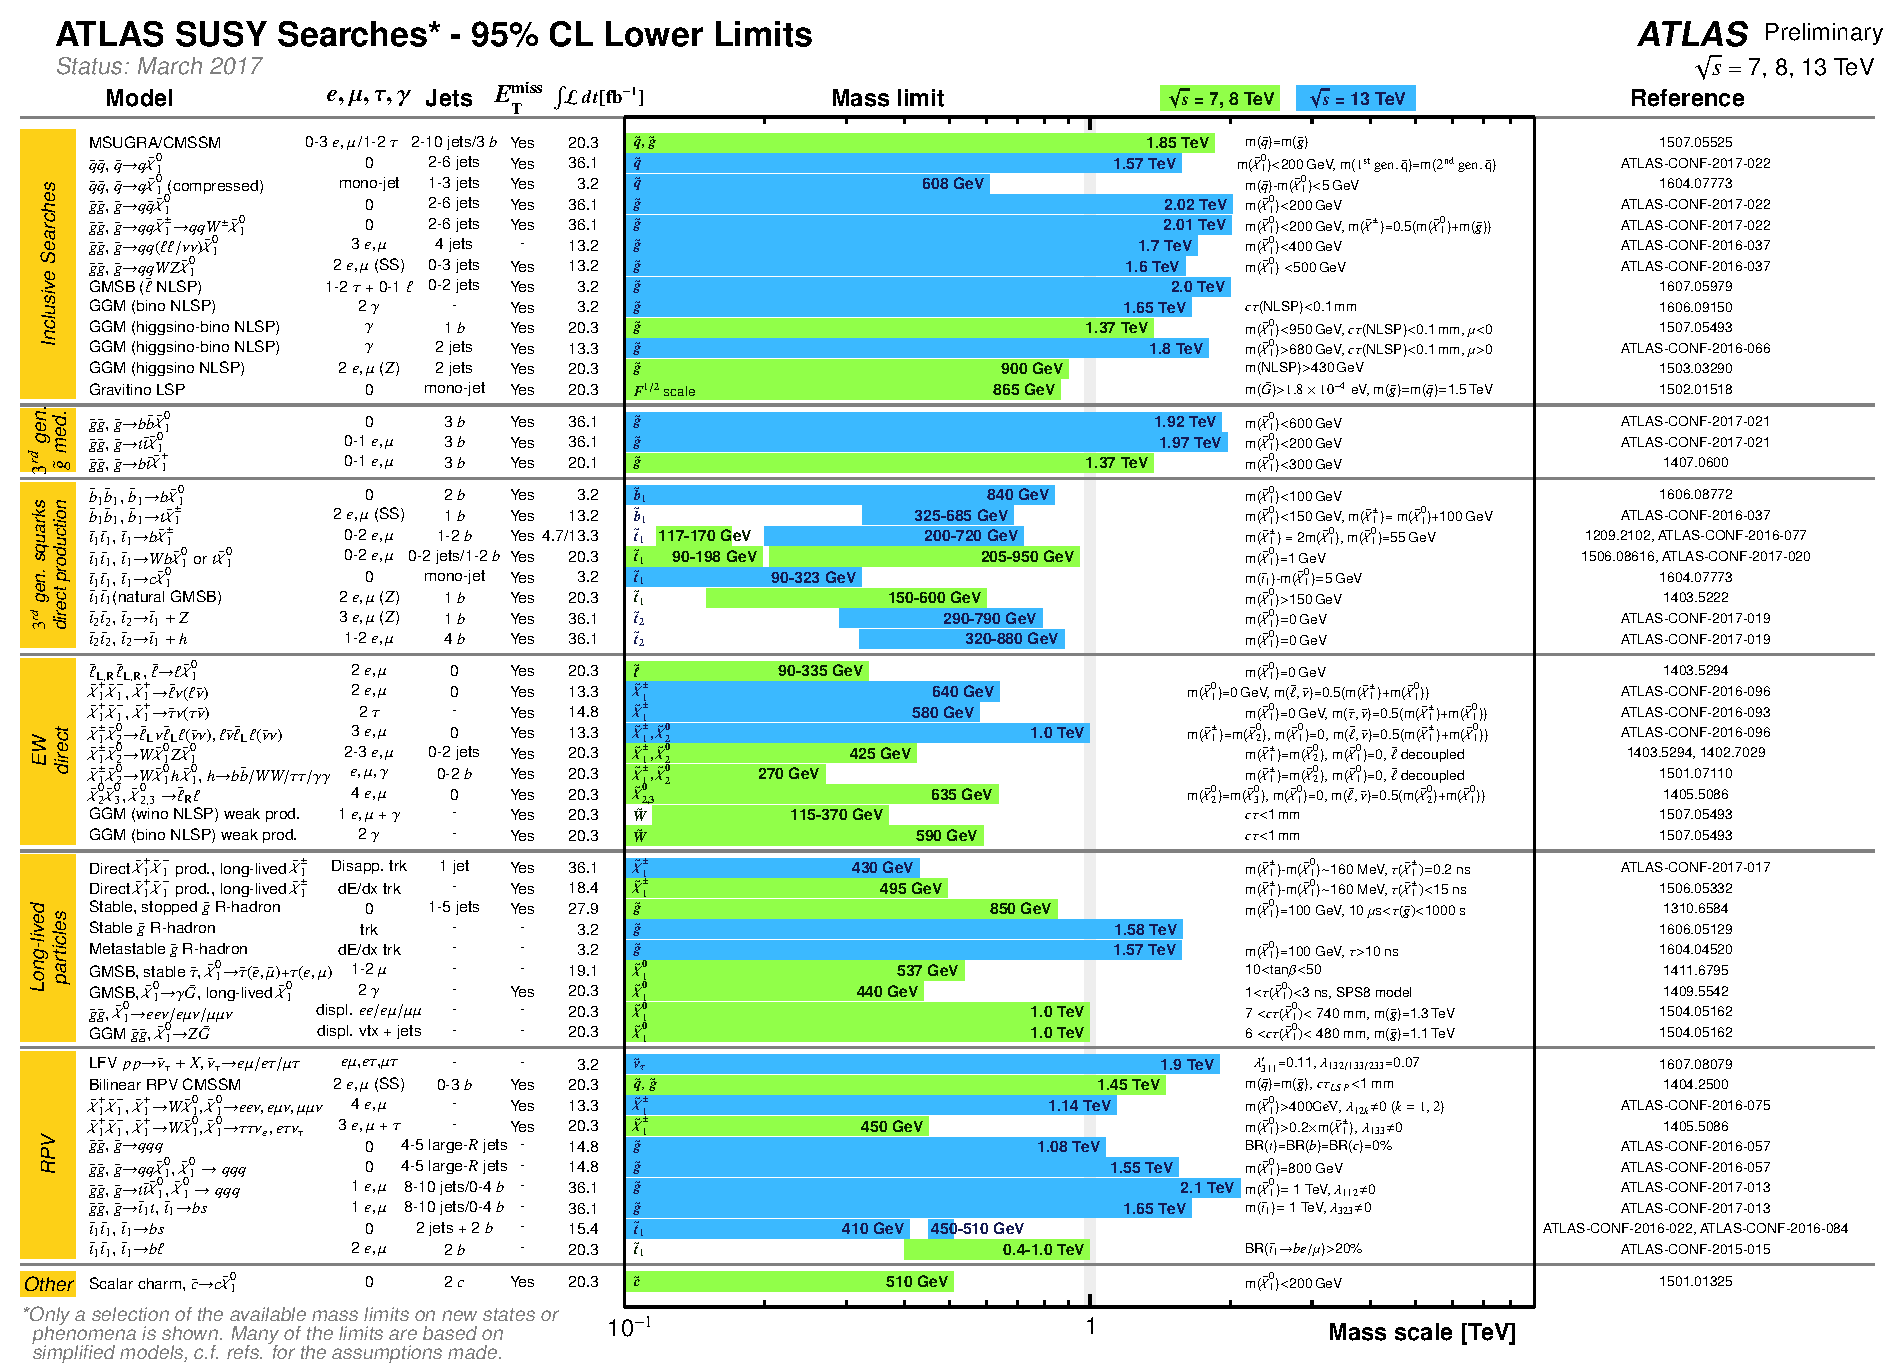
\includegraphics[width=1\textwidth]{masses.pdf}
\caption{Resumen de los límites de exclusión en la masa de las partículas supersimétricas por distintos análisis realizados en ATLAS \cite{masses_web}.}
\label{masses}
\end{figure}



\section{Colisión \textit{pp}}

El LHC es un colisionador de protones, por lo tanto para comprender los procesos que ocurren en el mismo, es necesario entender la estructura del protón. Su composición se puede describir mediante la cromodinámica cuántica (QCD) \cite{ellis1996}, que explica las interacciones entre partículas que poseen carga de color: quarks y gluones. Los mediadores de la interacción, los gluones, pueden interactuar consigno mismo, lo que produce que la fuerza dependa de la distancia entre las cargas. De esta forma, la constante de acoplamiento de la fuerza, aumenta a grandes distancias (o bajas energías) y disminuye para distancias menores (altas energías). Es por este motivo que los cálculos perturbativos solo se pueden efectuar a altas energías. Otra característica de la interacción es el confinamiento, es decir, que las partículas con color no puedan existir libremente. Solo estados de color neutro de múltiples partículas de color pueden ser observados en la naturaleza viajando distancias macroscópicas.

El protón es un barión, compuesto por dos quarks \textit{u} y un quark \textit{d}, cada uno con una carga de color tal que deje al protón en un estado neutro. Estos tres quarks son llamados quarks de valencia del protón, y están rodeados por un mar de gluones y pares de quark-antiquark que surgen de fluctuaciones cuánticas. A altas energías la colisión entre protones se puede considerar como una colisión entre dos de sus constituyentes, aplicando el <<modelo de partones>>. Este modelo fue introducido por Feynman \cite{PhysRevLett.23.1415} y Bjorken \cite{PhysRev.185.1975} a fines de los años 60, para interpretar los resultados de los experimentos de dispersión inelástica profunda (DIS) electrón-nucleón en SLAC. Los quarks de valencia y los quarks y antiquarks del mar junto con los gluones son llamados <<partones>> del protón. Cada partón lleva solo una fracción del momento y la energía del protón. Para la medición de una sección eficaz de dispersión fuerte que involucre quarks y gluones en el estado inicial, es necesario conocer el momento de las partículas incidentes. Como los partones solo llevan una fracción del momento del protón, y están en interacción permanente entre ellos, el momento es desconocido, por lo que la escala de energía de las colisiones varía. Además, como se mencionó, los quarks (\textit{q}) y gluones (\textit{g}) salientes no pueden observarse directamente debido al confinamiento, pero son observados en el detector como jets. Entonces no es posible medir una sección eficaz partónica como $\sigma(qg \rightarrow qg)$, pero se puede hacer una medida inclusiva, como la sección eficaz hadrónica $\sigma(pp \rightarrow jj)$ con dos jets en el estado final. En teoría de perturbaciones, para pasar desde la sección eficaz partónica a la sección eficaz hadrónica es necesario conocer la probabilidad de que un partón de tipo \textit{n} sea encontrado con una fracción de momento \textit{x}, es decir, las funciones de distribución partónica (PDF). Estas funciones son determinadas a partir de datos obtenidos de los propios experimentos de altas energías, ya que no pueden determinarse a partir de la teoría. 

Esta conexión entre los hadrones observables y el nivel partónico es posible gracias al concepto de <<factorización>>, que permite una separación sistemática entre las interacciones de corta distancia (de los partones) y las interacciones de larga distancia (responsables del confinamiento de color y la formación de hadrones). El teorema de factorización \cite{ELLIS1978281} establece que la sección eficaz de producción de cualquier proceso de QCD del tipo $A + B \rightarrow X$, siendo $a_{i}$ ($b_{j}$) los constituyentes del hadrón inicial $A$ ($B$), puede ser expresada como: 

\begin{equation}
\sigma_{AB\rightarrow X}=\sum_{ij}\int dx_{a_{i}}dx_{b_{j}}f_{A/a_{i}}(x_{a_{i}},\mu_{F}^{2})f_{B/b_{j}}(x_{b_{j}},\mu_{F}^{2})\sigma_{a_{i}b_{j}}(\mu_{F}^{2},\mu_{R}^{2})
\end{equation}

\noindent
donde $x_{i}$ ($x_{j}$) es la fracción del momento del hadrón $A$($B$) que lleva el partón $a_{i}$ ($b_{j}$) y $\sigma_{a_{i}b_{j}\rightarrow X}$ es la sección eficaz de la interacción a nivel partónico, calculada a un dado orden de perturbaciones y una escala de renormalización $\mu_R$. La escala de renormalización es introducida para absorber las divergencias ultravioletas que aparecen en los cálculos perturbativos más allá del primer orden. Las funciones $f_{A/a_{i}}(x_{a_{i}},\mu_{F}^{2})$ son las PDF, que representan la probabilidad de encontrar un partón de tipo \textit{n} en el hadrón \textit{h} con una fracción de momento $x_{n}$, dada una escala de factorización $\mu_{F}$. Esta escala es un parámetro arbitrario introducido para tratar singularidades que aparecen en el régimen no perturbativo. Estas divergencias son absorbidas, en forma similar a la renormalización, dentro de las funciones de distribución partónicas a la escala $\mu_{F}$. 


A modo de ejemplo, en la Figura \ref{cross_section}, se muestra el buen acuerdo entre la sección eficaz de algunos procesos del SM medidas por ATLAS y las predicciones teóricas. Las observaciones experimentales realizadas en LHC resultan compatibles con el SM a un nivel de muy alta precisión.


\begin{figure}[ht]
\centering
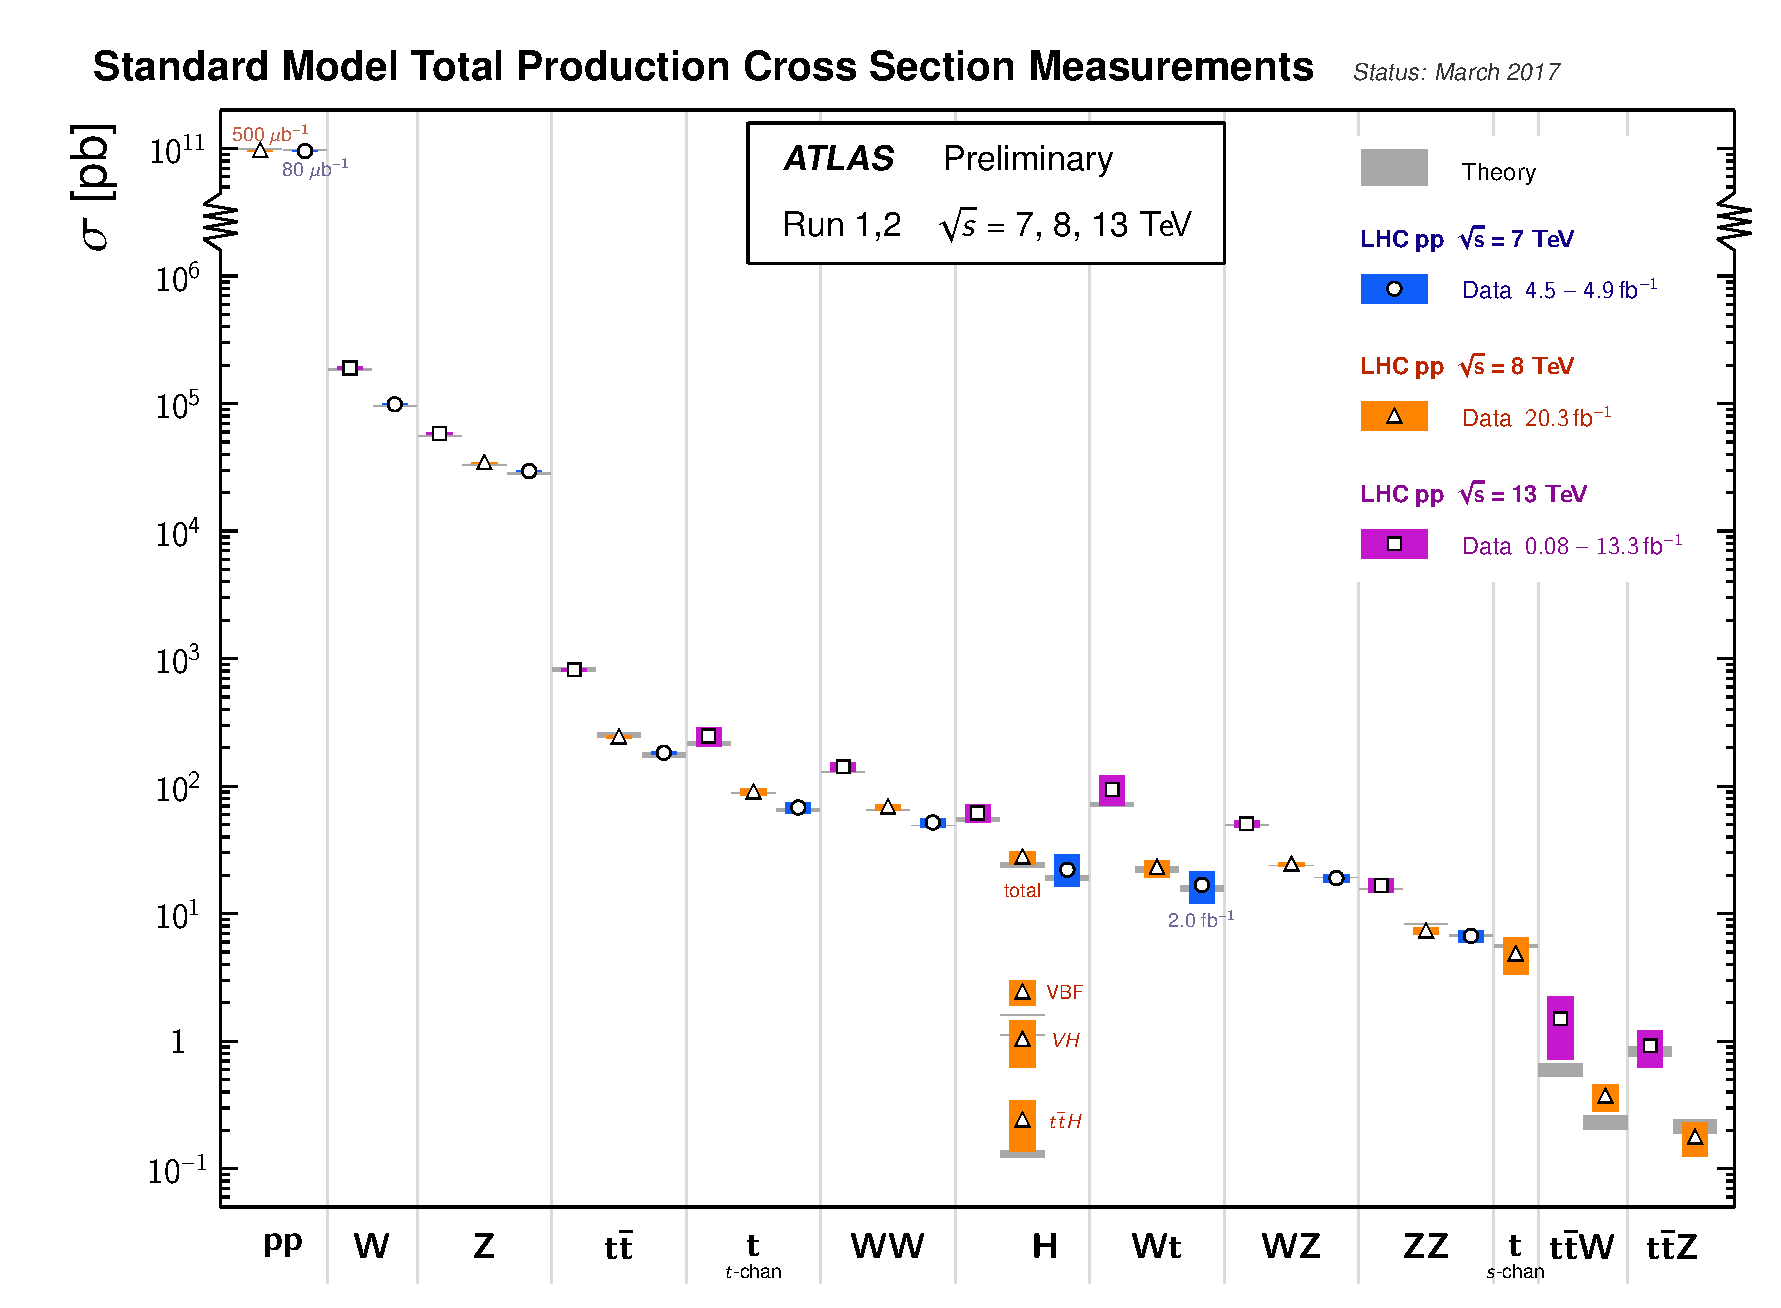
\includegraphics[width=1\textwidth]{cross_section.pdf}
\caption{Resumen de las distintas medidas de sección eficaz de producción de procesos del SM, comparadas con sus valores teóricos esperados \cite{crosssect_web}.}
\label{cross_section}
\end{figure}


\clearpage

\chapter{El LHC y el detector ATLAS}
% \addcontentsline{toc}{chapter}{El LHC y el detector ATLAS}
\chaptermark{El LHC y el detector ATLAS}


El Gran Colisionador de Hadrones (\textit{\textbf{L}arge \textbf{H}adron \textbf{C}olider} (LHC)) \cite{Evans:1129806} es el acelerador de hadrones del Centro Europeo para la Investigación Nuclear (CERN), ubicado en la frontera entre Francia y Suiza. Posee una longitud de 27 km y fue construido en el mismo túnel en el que funcionaba el acelerador $e^{+}e^{-}$ LEP (etre 1989 y 2000), a una profundidad variable entre $50$ y $174$ m de la superficie.

El LHC está diseñado para colisionar protones (e iones pesados) a una energía de centro de masa de $\sqrt{s}=14$ TeV. Para ello el CERN posee un complejo de aceleradores que, en sucesivas etapas, incrementan la energía de los protones (Figura \ref{acc_complex}). El último de los aceleradoes es el LHC, donde los protones circulan en direcciones opuestas por cavidades de ultra alto vacío a una presion de $10^{-10}$ torr. El mismo cuenta con $1232$ dipolos magnéticos superconductores enfriados a $1.9$ K, que generan un campo magnético de $8.4$ T, lo que permitemantener en su órbita circular a los protones. Los dipolos están equipados con sextupolos, octupolos y decapolos, que permiten corregir las pequeñas imperfecciones del campo magnético en las extermiadesde de los dipolos. Para aumentar la probabildiad de colisión, existe un sistema de focalización de los haces en las proximidades de los detectores, que estrecha el camino que recorren los protones. El mismo consiste de $392$ cuadrupolos magnéticos que generan campos magnéticos de $6.8$ T. 

\begin{figure}[ht]
\centering
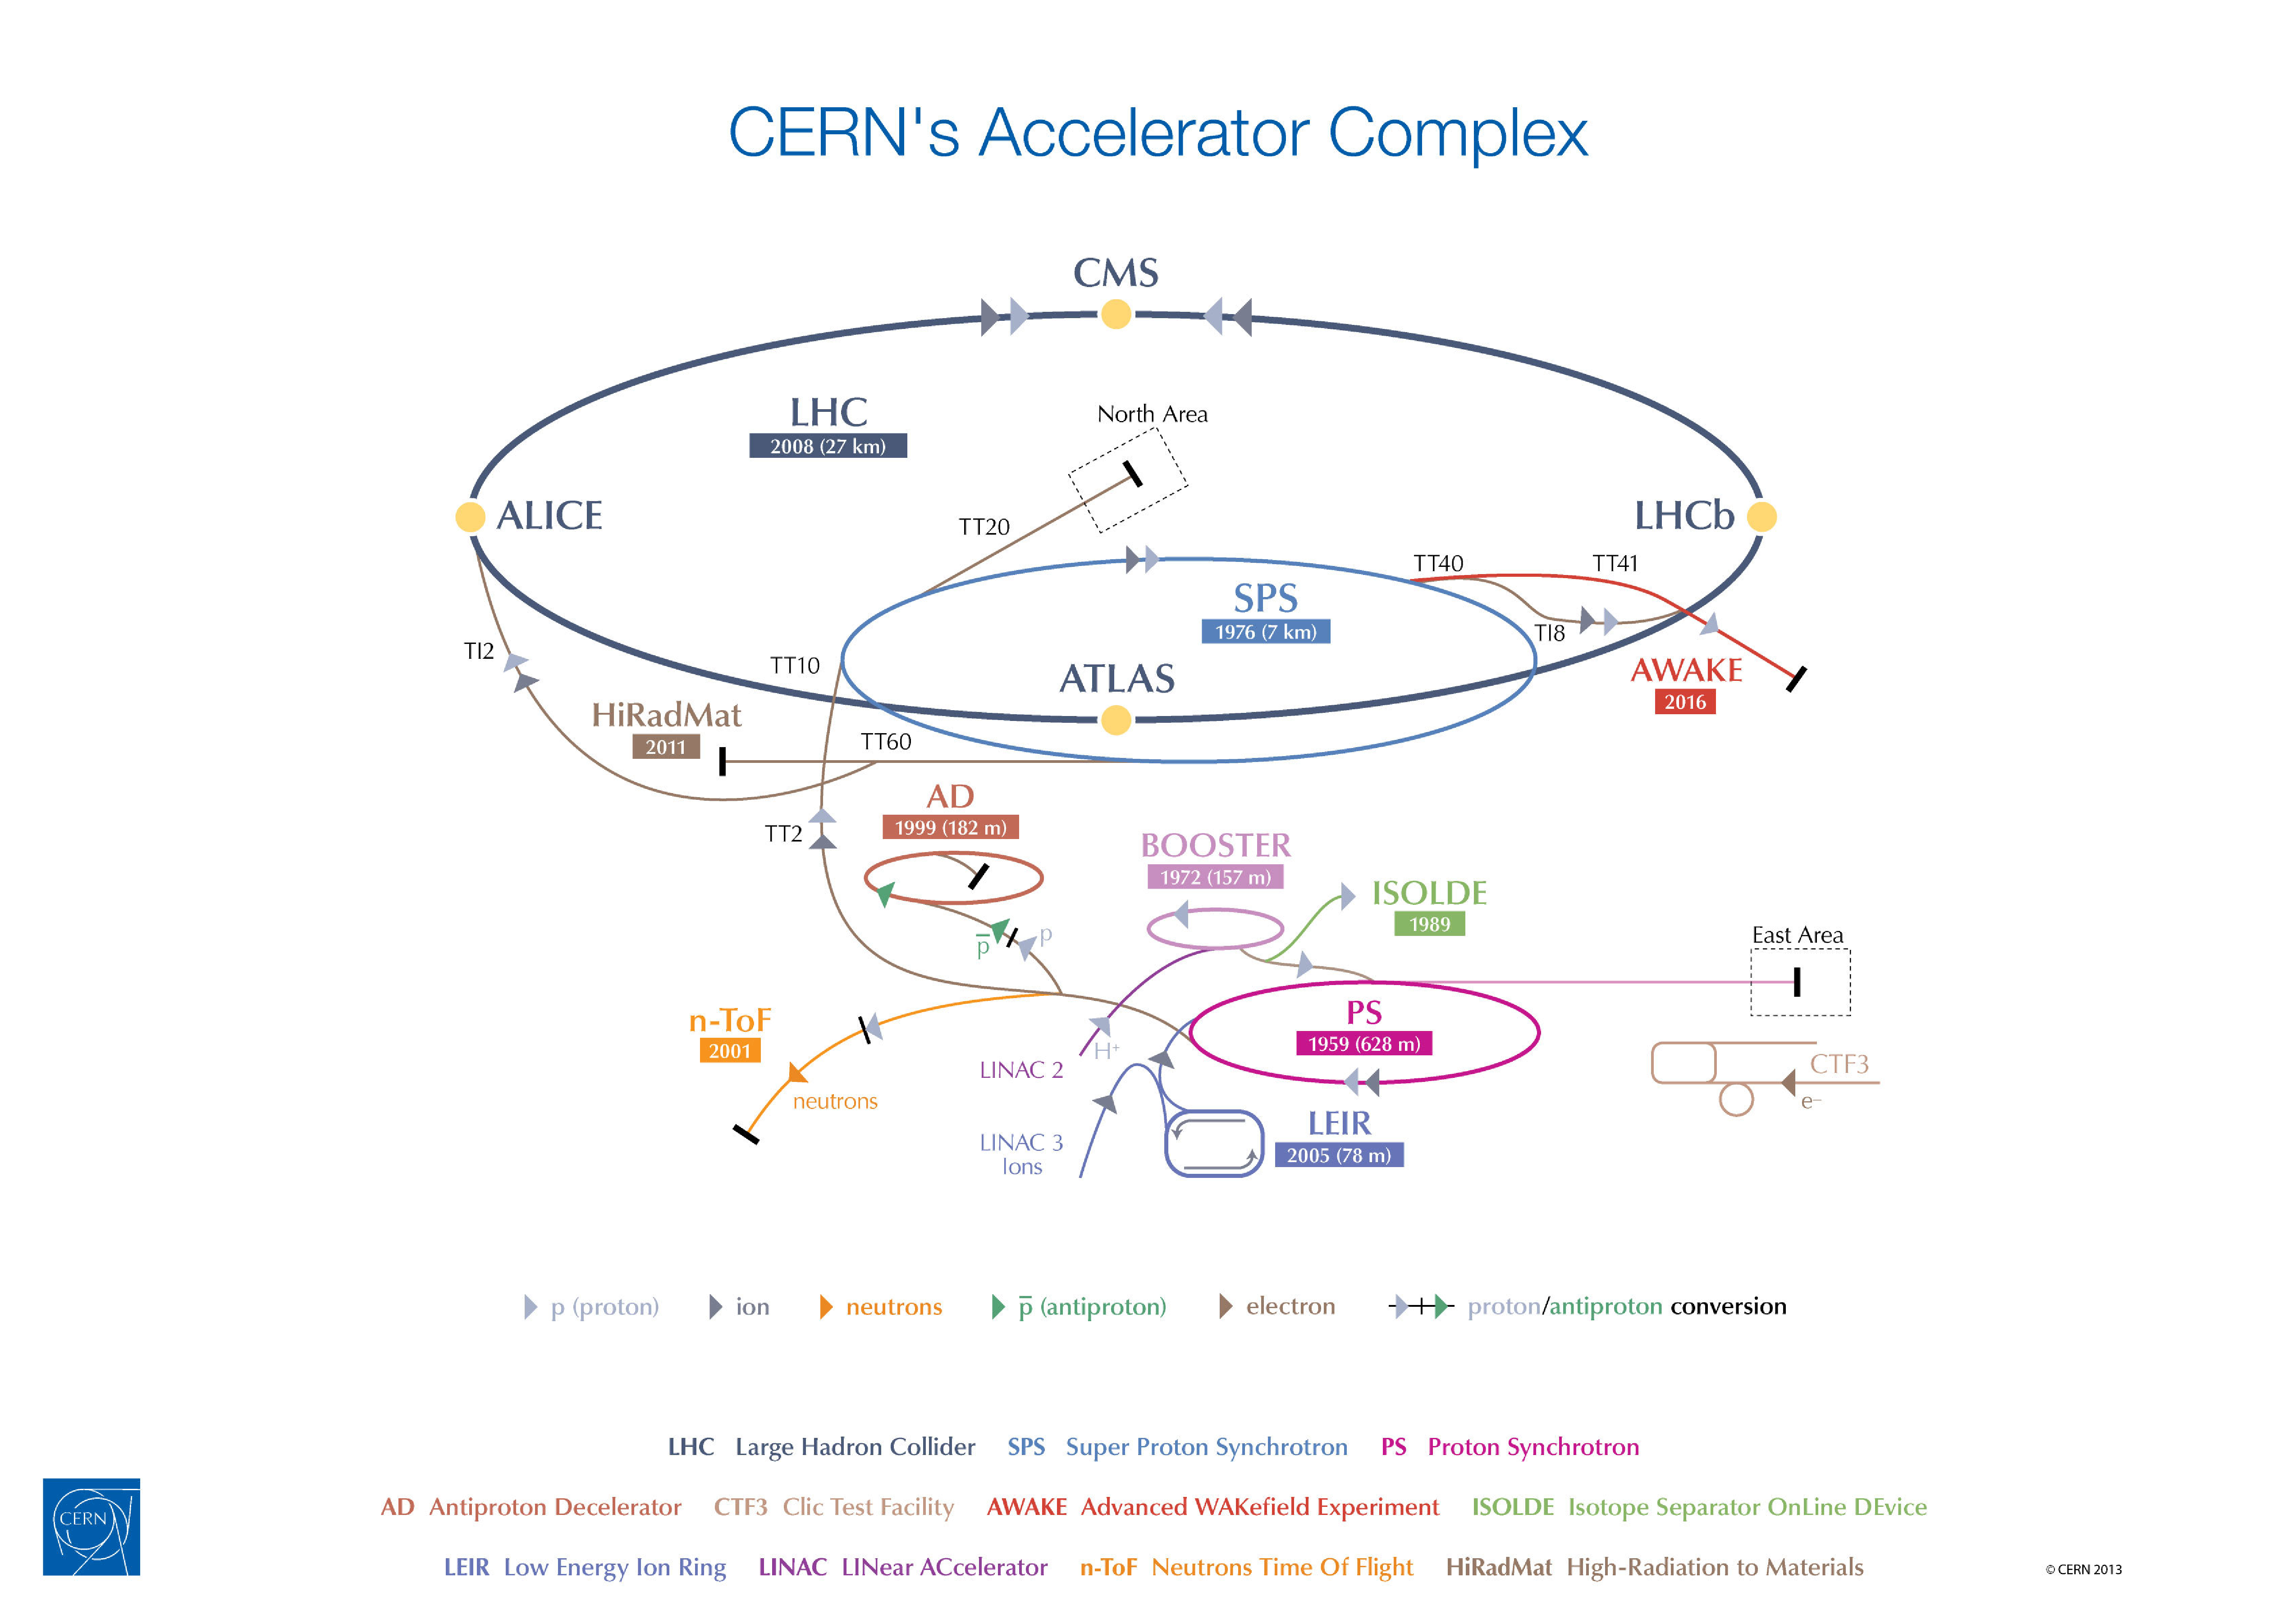
\includegraphics[width=1\textwidth]{acc_complex.eps}
\caption{Complejo de aceleradores del CERN, incluyendo al LHC y a la serie de aceleradores utilizados para proveer de protones al LHC. También pueden verse los diferentes experimentos ubicados en distintos puntos del acelerador.}
% \vspace{0.2cm}\footnotesize\textbf \sl{...}\vspace{0.2cm}
\label{acc_complex}
\end{figure}

El diseño del LHC contempla trenes de $2808$ paquetes de $\sim 10^{11}$ protones cada uno, espaciados temporalmente en $25$ ns. Para caracterizar el funcionamiento del acelerador, se utiliza una varaible denominada luminosidad instantánea. Se define como el número de partículas por unidad de tiempo y unidad de área:

\begin{equation}
\mathcal{L}=f_{rev}n_{b}\frac{N_{1}N_{2}}{A}
\end{equation}

donde $f_{rev}$ es la frecuencia de revolución ($\sim$ 11 kHz), $n_{b}$ es el número de \textit{bunches} (paquetes de protones) por haz, $N_{i}$ es el número de partículas en cada \textit{bunch} y \textit{A} es la sección efectiva del haz, que puede expresarse en término de los parámetros del acelerador como:

\begin{equation}
A=\frac{4 \pi \epsilon_{n}\beta^{*}}{\gamma F}
\end{equation}

donde $\epsilon_{n}$ es la emitancia transversal normalizada (la dispersión transversal media de las partículas del  haz en el espacio de coordenadas e impulsos), $\beta^{*}$ es la función de amplitud en el punto de interacción, relacionada al poder de focalización de los cuadrupolos), $\gamma$ es el factor relativista de Lorentz y \textit{F} es un factor de reducción geométrico, debido al ángulo de cruce de los haces en el punto de interacción.

... Datos actuales

\section{El detector ATLAS}

ATLAS (\textit{\textbf{A} \textbf{T}oroidal \textbf{L}HC \textbf{A}paratu\textbf{S}})  \cite{PERF-2007-01} es uno de los experimentos multipropósito del LHC, diseñado para estudiar las colisiones protón-protón a altas energías provistas por el LHC.

El esquema del detector se puede observar en la Figura \ref{ATLAS}. Tiene una smietría aproximadamente cilíndrica, y está compuesto de distintos subdetectores que cumplen diversas funciones (ver Figura \ref{cross_section_2}). En la zona más próxima al haz se encuentra detector interno de trazas (ID), compuesto del Insertable B-Layer (IBL), un detector de píxeles, un detector de bandas de silicio (SCT) y un detector de radiación de transición (TRT). Envolviendo el ID se encuentra un solenoide superconductor que genera un campo magnético de $2$ T, el cual curva la trayectoria de las partículas cargadas para así medir su impulso.

\begin{figure}
\centering
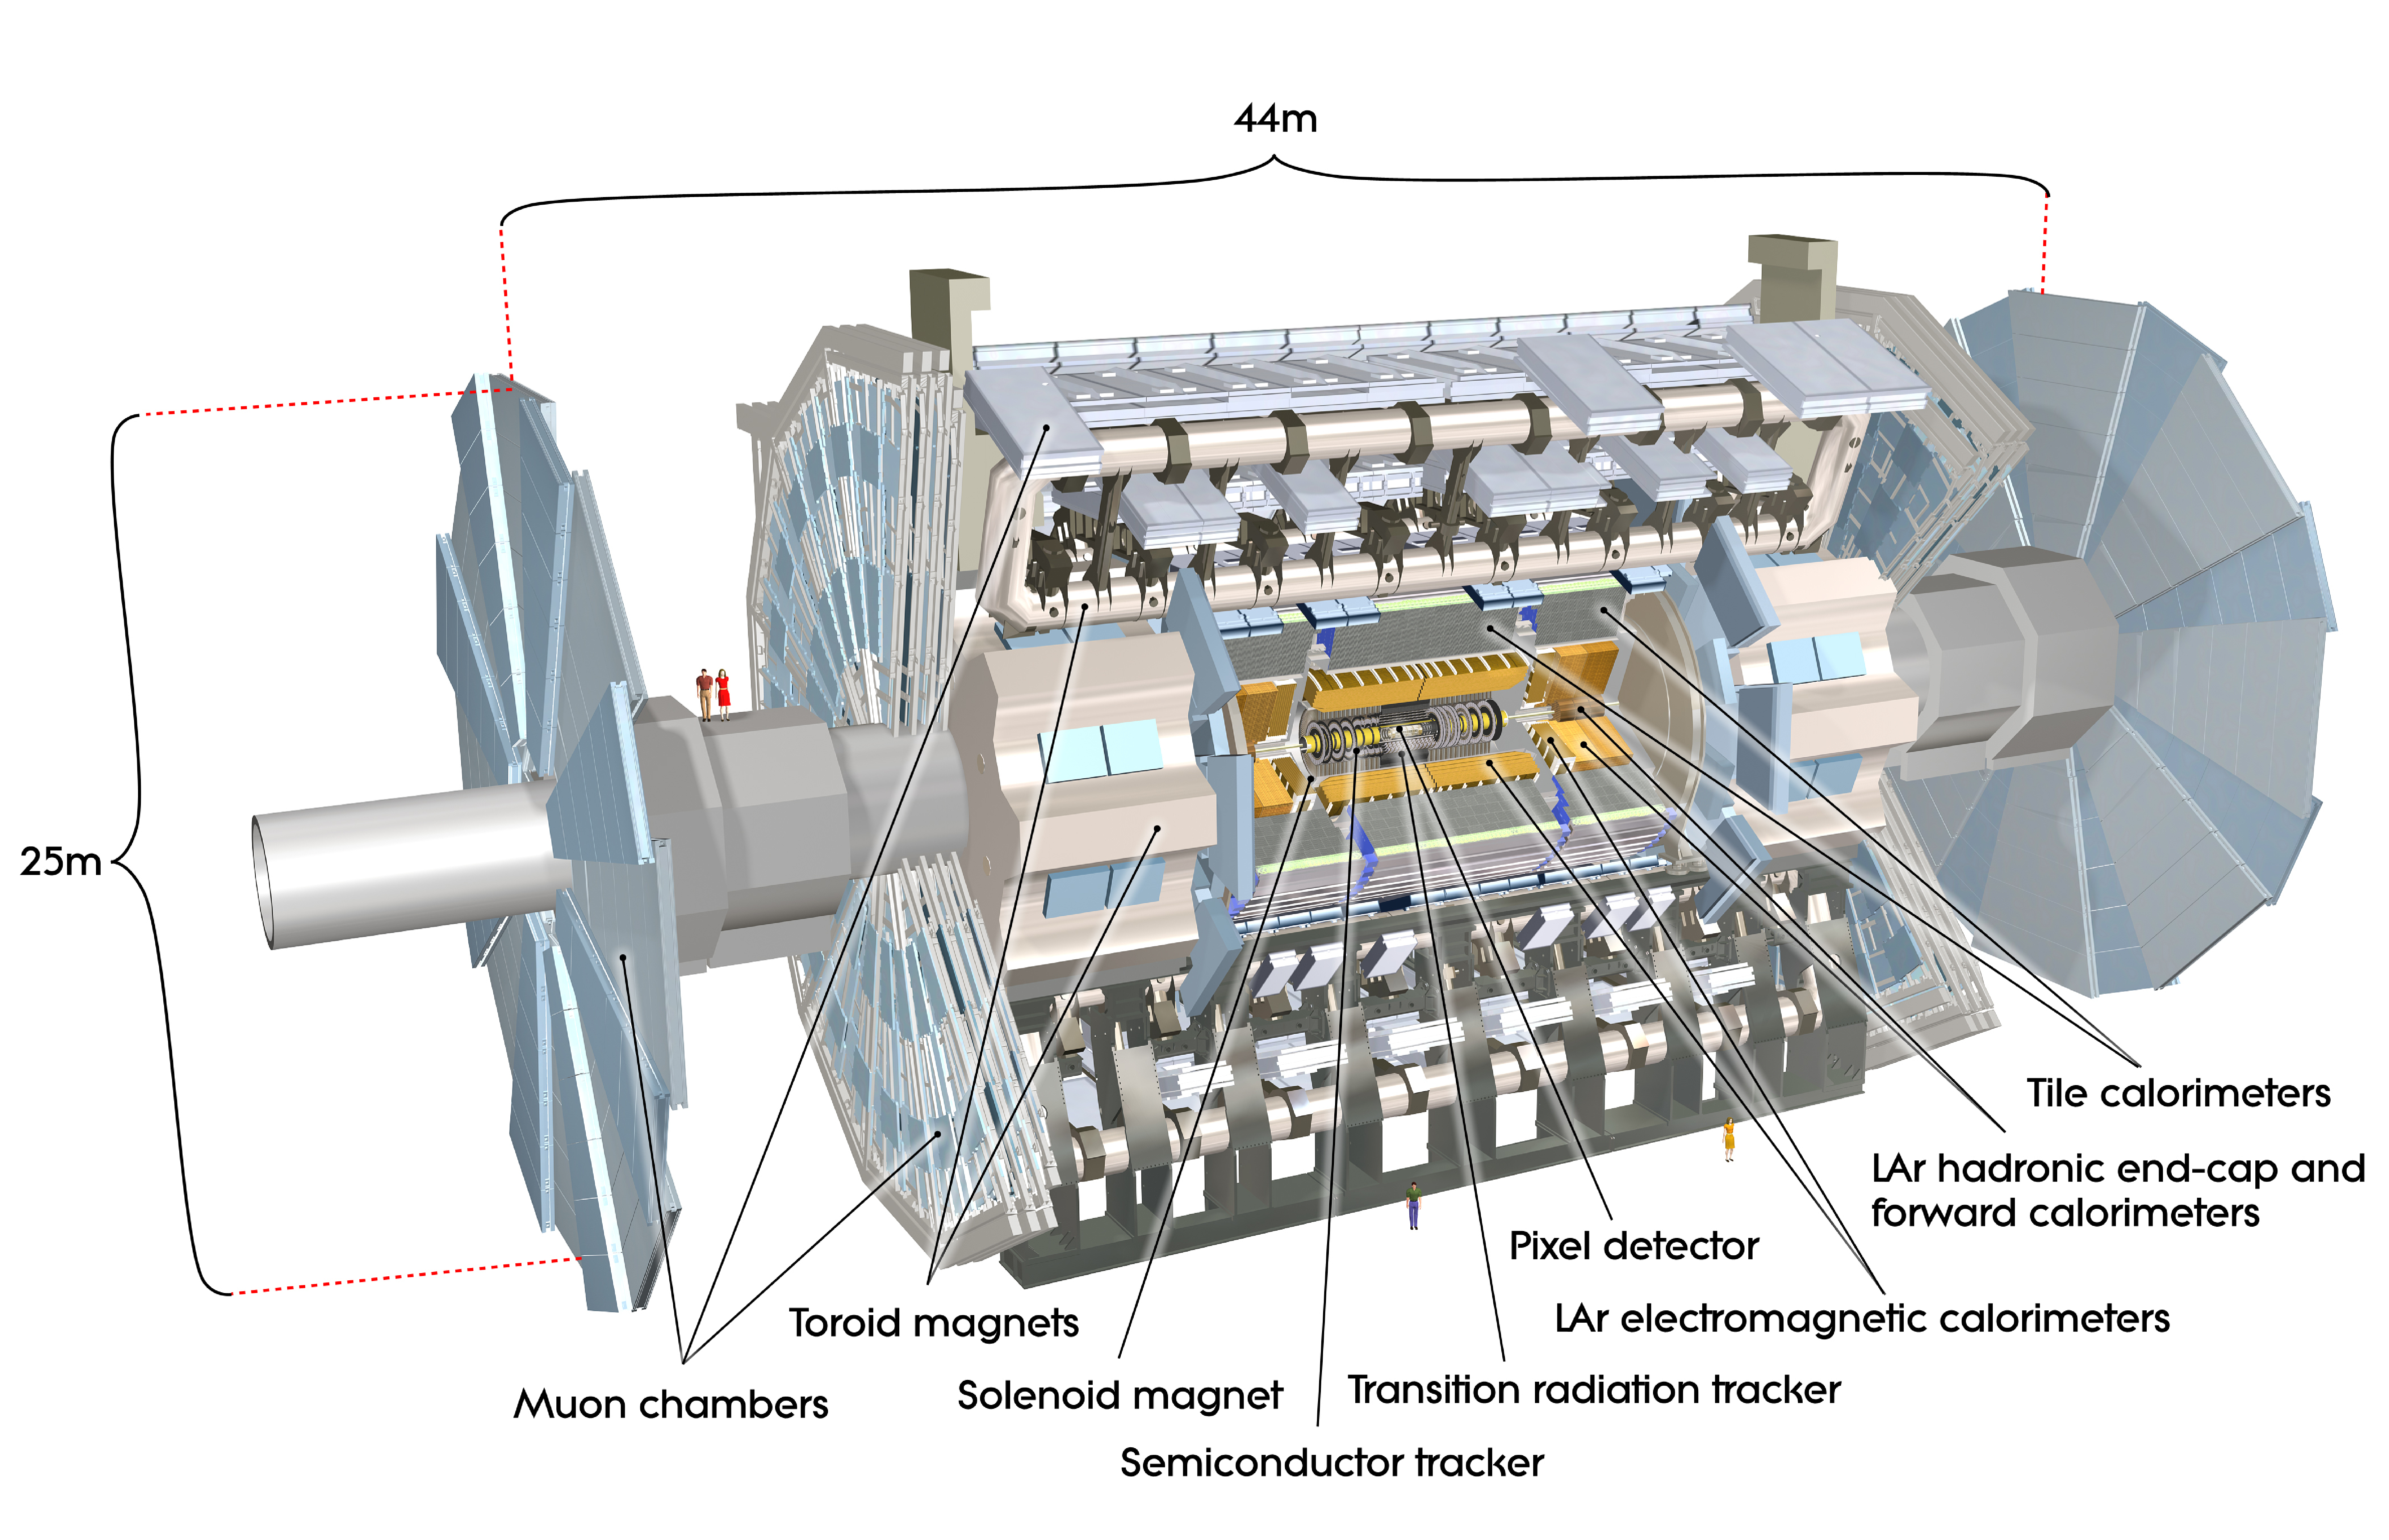
\includegraphics[width=1\textwidth]{ATLAS.eps}
\caption{Esquema general del detector de ATLAS.}
% \vspace{0.2cm}\footnotesize\textbf \sl{...}\vspace{0.2cm}
\label{ATLAS}
\end{figure}

\begin{figure}
\centering

\includegraphics[width=0.7\textwidth]{cross_section_2.eps}
\caption{Esquema del corte transversal del detector de ATLAS, ilustrando los distintos subdetectores y el pasaje de los distintos tipos de partículas.}
% \vspace{0.2cm}\footnotesize\textbf \sl{...}\vspace{0.2cm}
\label{cross_section_2}
\end{figure}

A continuación se ubica el sistema de calorímetros: el calorímetro electromagnético (ECAL) que mide la energía depositada por fotones y electrones, y el calorímetro hadrónico (HCAL) para medir la energía de los jets y hadrones.

Finalmente, se encuetra el espectrómetro de muones (MS) intercalado con un sistema de imanes toroidales, que generan un campo magnetico necesario apra curvar la trayectoria de los muones dentro del detector.

El detector ATLAS se divide geométricamente en dos regiónes, la parte central denominada \textit{barrel} y la región extrema \textit{endcap}. En la región \textit{barrel} los detectores se ubican en forma de cilindros concentricos alrededor del eje del haz, mientras en la región \textit{endcap} se disponen como discos perpendiculares a la dirección del haz. 

\section{Sistema de coordenadas}

El sistema de coordenadas de ATLAS corresponde a un sistema cartesiano, cuyo origen coincide con el punto de interacción nominal. El eje \textit{z} corresponde al eje del haz, el eje \textit{x} se define desde el punto de interacción hacia el centro del LHC, y el eje \textit{y} se define apuntando hacia arriba.

Es conveniente además definir un sistema de coordenadas cilíndricas. Donde el radio \textit{R} representa la distancia perpendicular al haz. El ángulo azimutal $\phi$ es medido alrededor del eje del haz, y el ángulo $\theta$ se mide con respecto al eje del haz. 

Una cantidad muy importante utilizada en física de altas energías es la llamada rapidez:

\begin{equation}
w=\frac{1}{2}\ln\left( \frac{E+p_{z}}{E-p_{z}}\right)
\end{equation}

donde \textit{E} es la energía total de la partícula y $p_{z}$ es la componente longitudinal de su impulso. En el límite de altas energías esta cantidad se aproxima (en forma exacta para objetos no masivos) por la llamada pseudorapidez, $\eta$, relacionada con el ángulo polar $\theta$ como:

\begin{equation}
\eta =-\ln \tan\left( \frac{\theta}{2} \right)
\end{equation}

La razón detrás de esta transformación de coordenadas es el hecho que la multiplicidad de partículas producidas es aproximadamente constante como función de $\eta$, y que la diferencia de pseudorapidez entre dos partículas es invariante frente a transformaciones de Lorentz a lo largo de la dirección del haz. 

En el caso de colisiones hadrónicas, la fracción del impulso del protón adquirida por cada uno de las partones interactuantes es desconocida. Parte de este impulso es transferido en la interacción dura, mientras cierta fracción remanente escapa el detector a lo largo del haz. Así, no es posible reconstruir el movimiento longitudinal del centro de masa en la interacción, y aplicar leyes de conservación sobre la cinemática de cada evento. Sin embargo, dado que los protones inciden a lo largo de la dirección del haz, y asumiendo que el momento transverso de los partones es nulo, el impulso total transverso se conserva durante la colisión. Por esta razón, solo las componentes transversales son utilizadas en la descripción de la cinemática del evento, por ejemplo $p_{T}$ ($=p\sin\theta$). En términos de la pseudorapidez, se define la energía transversa ($E_{T}=E\sin\theta$) de una partícula como:

\begin{equation}
E_{T}=\frac{E}{\cosh \eta}
\end{equation}

donde \textit{E} es su energía total.

\section{Los subdetectores de ATLAS}

\subsection{El detector interno}

\begin{figure}
\centering
\includegraphics[width=0.70\textwidth]{ID.eps}
\caption{Esquema general del detector interno de ATLAS.}
% \vspace{0.2cm}\footnotesize\textbf \sl{...}\vspace{0.2cm}
\label{ID}
\end{figure}

El detector interno es el más próximo al haz y esta contenido dentro de un solenoide que provee un campo magnetico de $2$ T. Un esquema general del mismo se puede observar en la figura \ref{ID}. Está compuesto por distintos detectores como muestra la figura \ref{ID_2}.

\begin{figure}
\centering
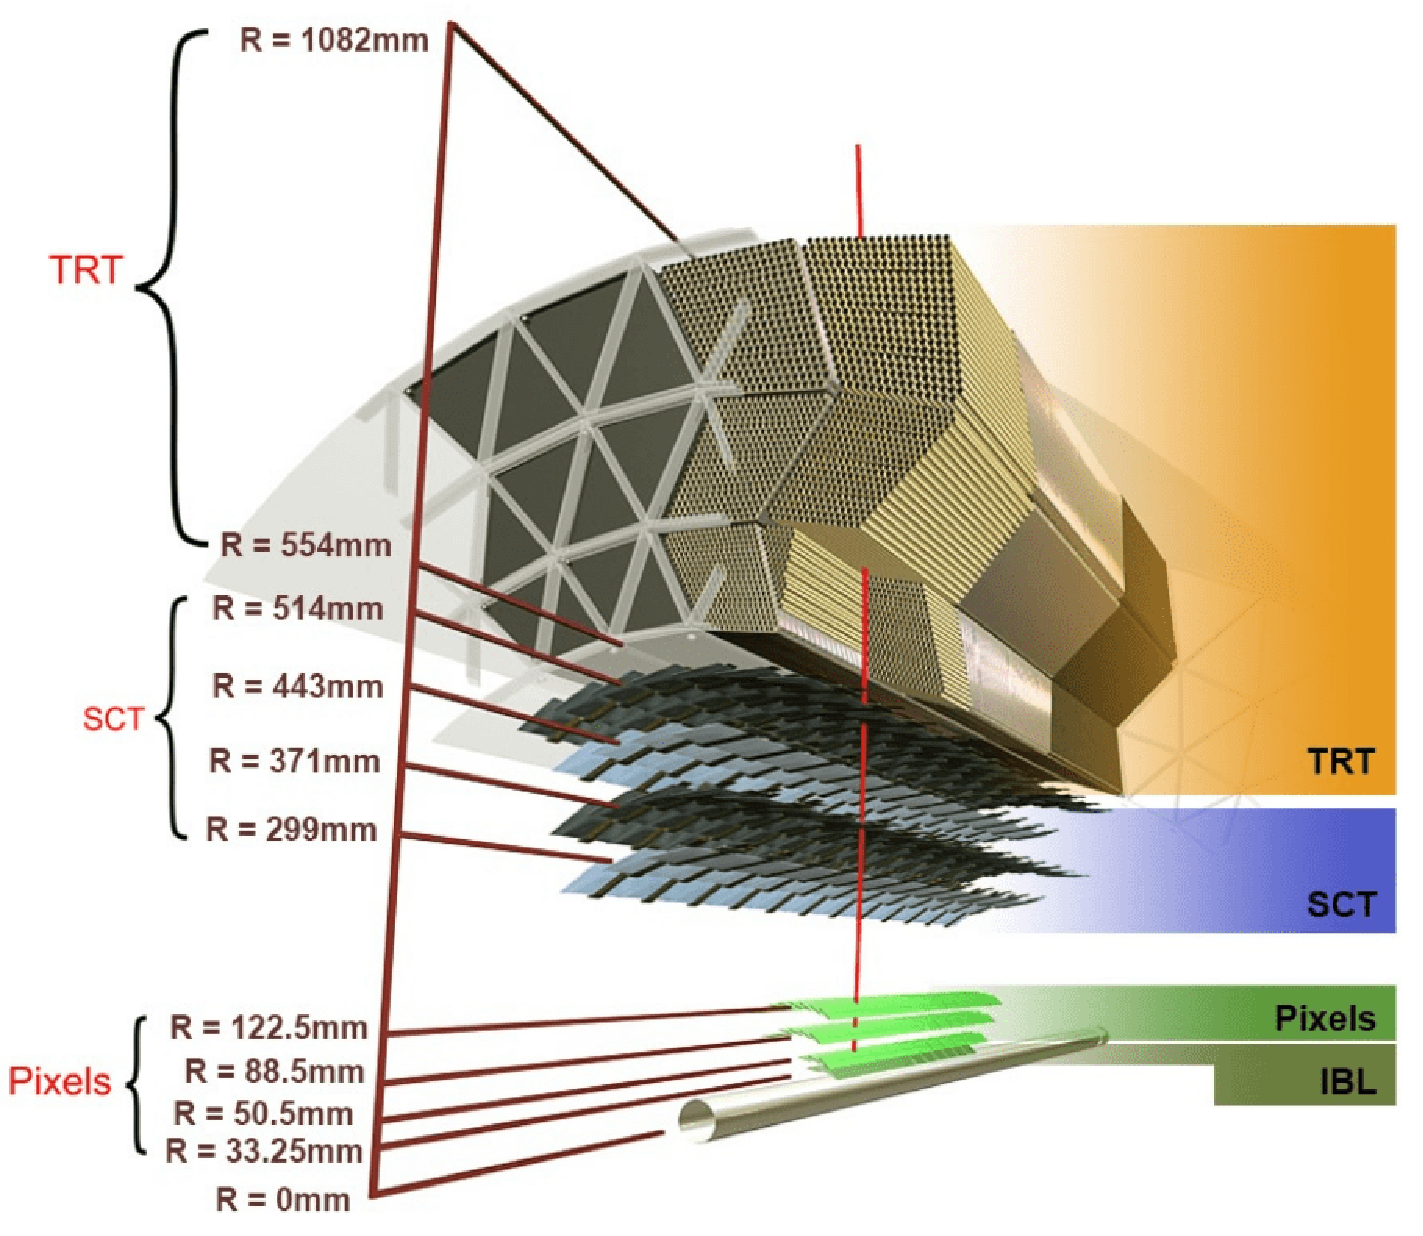
\includegraphics[width=0.60\textwidth]{ID_2.eps}
\caption{Esquema del detector interno mostrando la traza de una partícula cargada de $p_{T}=10\egev$ atravesándolo. La trayectoria atraviesa el tubo del haz de  erilio, las tres capas del detector de píxeles de silicio (Pixels), las cuatro capas dobles de sensores semiconductores (SCT), y aproximadamente 36 tubos contenidos en los módulos del detector por radiación de transición (TRT).}
% \vspace{0.2cm}\footnotesize\textbf \sl{...}\vspace{0.2cm}
\label{ID_2}
\end{figure}
\vspace{0.5cm}

{\bf Insertable B-Layer}

PUEDE IR AL FINAL?

Luego del Run 1 la luminosidad del LHC aumentó notablemente, lo que podía significar un daño por radiación en los detectores internos. En vez de reemplazar las partes del detector de píxeles que podían ser dañadas, se decidió colocar una capa insertable entre el detector de píxeles y el tubo?. El objetivo principal del mismo es no perder eficiencia en la identificación del decaimiento de bottom quarks.

La distancia entre el IBL y el tubo es de $0.2$ mm, y entre el IBL y el detector de píxeles es de $1.9$ mm. El mismo esta compuesto de chips de rápida lectura y con con sensores de silicio, que detecta el paso de partículas cargadas mediante la deposición de carga inducida. El tamaño de los pixel es de $50$ $\mu$m, 5 veces menor que en el detector de píxeles.

\vspace{0.5cm}

{\bf Detector de píxeles }

El detector de píxeles fue construído para medir la posición de las trazas de partículas cargadas con la más alta precisión posbile y es de vital importancia para la reconstrucción de los vértices primarios y secundarios. En la región \textit{barrel} consiste en tres cilindros, mientras que la \textit{endcap} tres discos. El principio de detección para partículas cargadas es la medida de la deposición de la carga inducida en una capa de silicio por ionización. El sistema contiene un total de $80.4$ millones de sensores, cada uno con una resolucion intrínseca de entre $12$ $\mu$m y $110$ $\mu$m. AGREGAR IBL.

\vspace{0.5cm}

{\bf Detector Semiconductor de Trazas (SCT) }

Se encuentra por fuera del detector de píxeles y está deseñado para medir las trazas con alta precisión en la zona intermedia del detector. A diferencia del detector de píxeles, estos sensores de silicio están segmentados en micro bandas, dada la mas baja multiplicidad de partículas. La resolución varía entre $16$ $\mu$m y $580$ $\mu$m. En la región \textit{barrel} los módulos de SCT estan dispuestos en 4 capas concéntricas, mientras que en la región \textit{endcap} consiste en 9 discos transversales al eje del haz.

\vspace{0.5cm}

{\bf Detector de Radiación de Transición (TRT) }

Es el detector más externo del ID y está diseñado, no solo para detectar partículas cargadas, sino también para detectar la radiación de transición que permite distinguir entre partículas cargadas pesadas y livianas (diferenciar entre $\pi^{\pm}$ y $e^{\pm}$ por ejemplo). El TRT se basa en el uso de tubos detectores que pueden operar a alta frecuencia de eventos gracias a su pequeño diámetro ($4$ mm) y el aislamiento de sus hilos centrales en volúmenes de gas individuales. La región barrel contiene $50000$ tubos paralelos al eje del haz y la región endacap $420000$ tubos orientados radialmente. Su resolucion es de $0.17$ mm. EXPLICAR POR QUE RADIACION.

\subsection{Calorímetros}

El sistema de calorímetros de ATLAS está sdiseñado para medir la energía y la posición de las partículas, mediante la absorción de la energía depositada por las cascadas de partículas secundarias que estas generan en el material del mismo. Además, permite discriminar electrones y fotones de jets, medir el desbalance de energía transversa y la selección online de eventos potencialmenteinteresantes (\textit{trigger}). Este sistema incluye un calorímetro electromagnético (ECAL) y otro hadrónico (HCAL), como muestra la figura \ref{Cal}.

\begin{figure}
\centering
\includegraphics[width=0.70\textwidth]{Cal.eps}
\caption{Sistema de calorímetros del detector ATLAS.}
% \vspace{0.2cm}\footnotesize\textbf \sl{...}\vspace{0.2cm}
\label{Cal}
\end{figure}

{\bf Calorímetro electromagnético }

La región \textit{barrel} de este sistema consiste en un calorímetros de muestreo que utiliza plomo como material absorbente. Las partículas incidentes iteractúan con este material, creando una lluvia de partículas cargadas y neutras. Las partículas cargadas ionizan el medio activo (LAr) colocado entra las placas de plomo, donde los electrones liberados son colectados en un electrodo central de kaptón/Cu hacia donde derivan por acción del campo eléctrico aplicado. La señal total en el medio activo es así poroporcional a la energía total real de la partícula incidente.

% \begin{figure}
% \centering
% 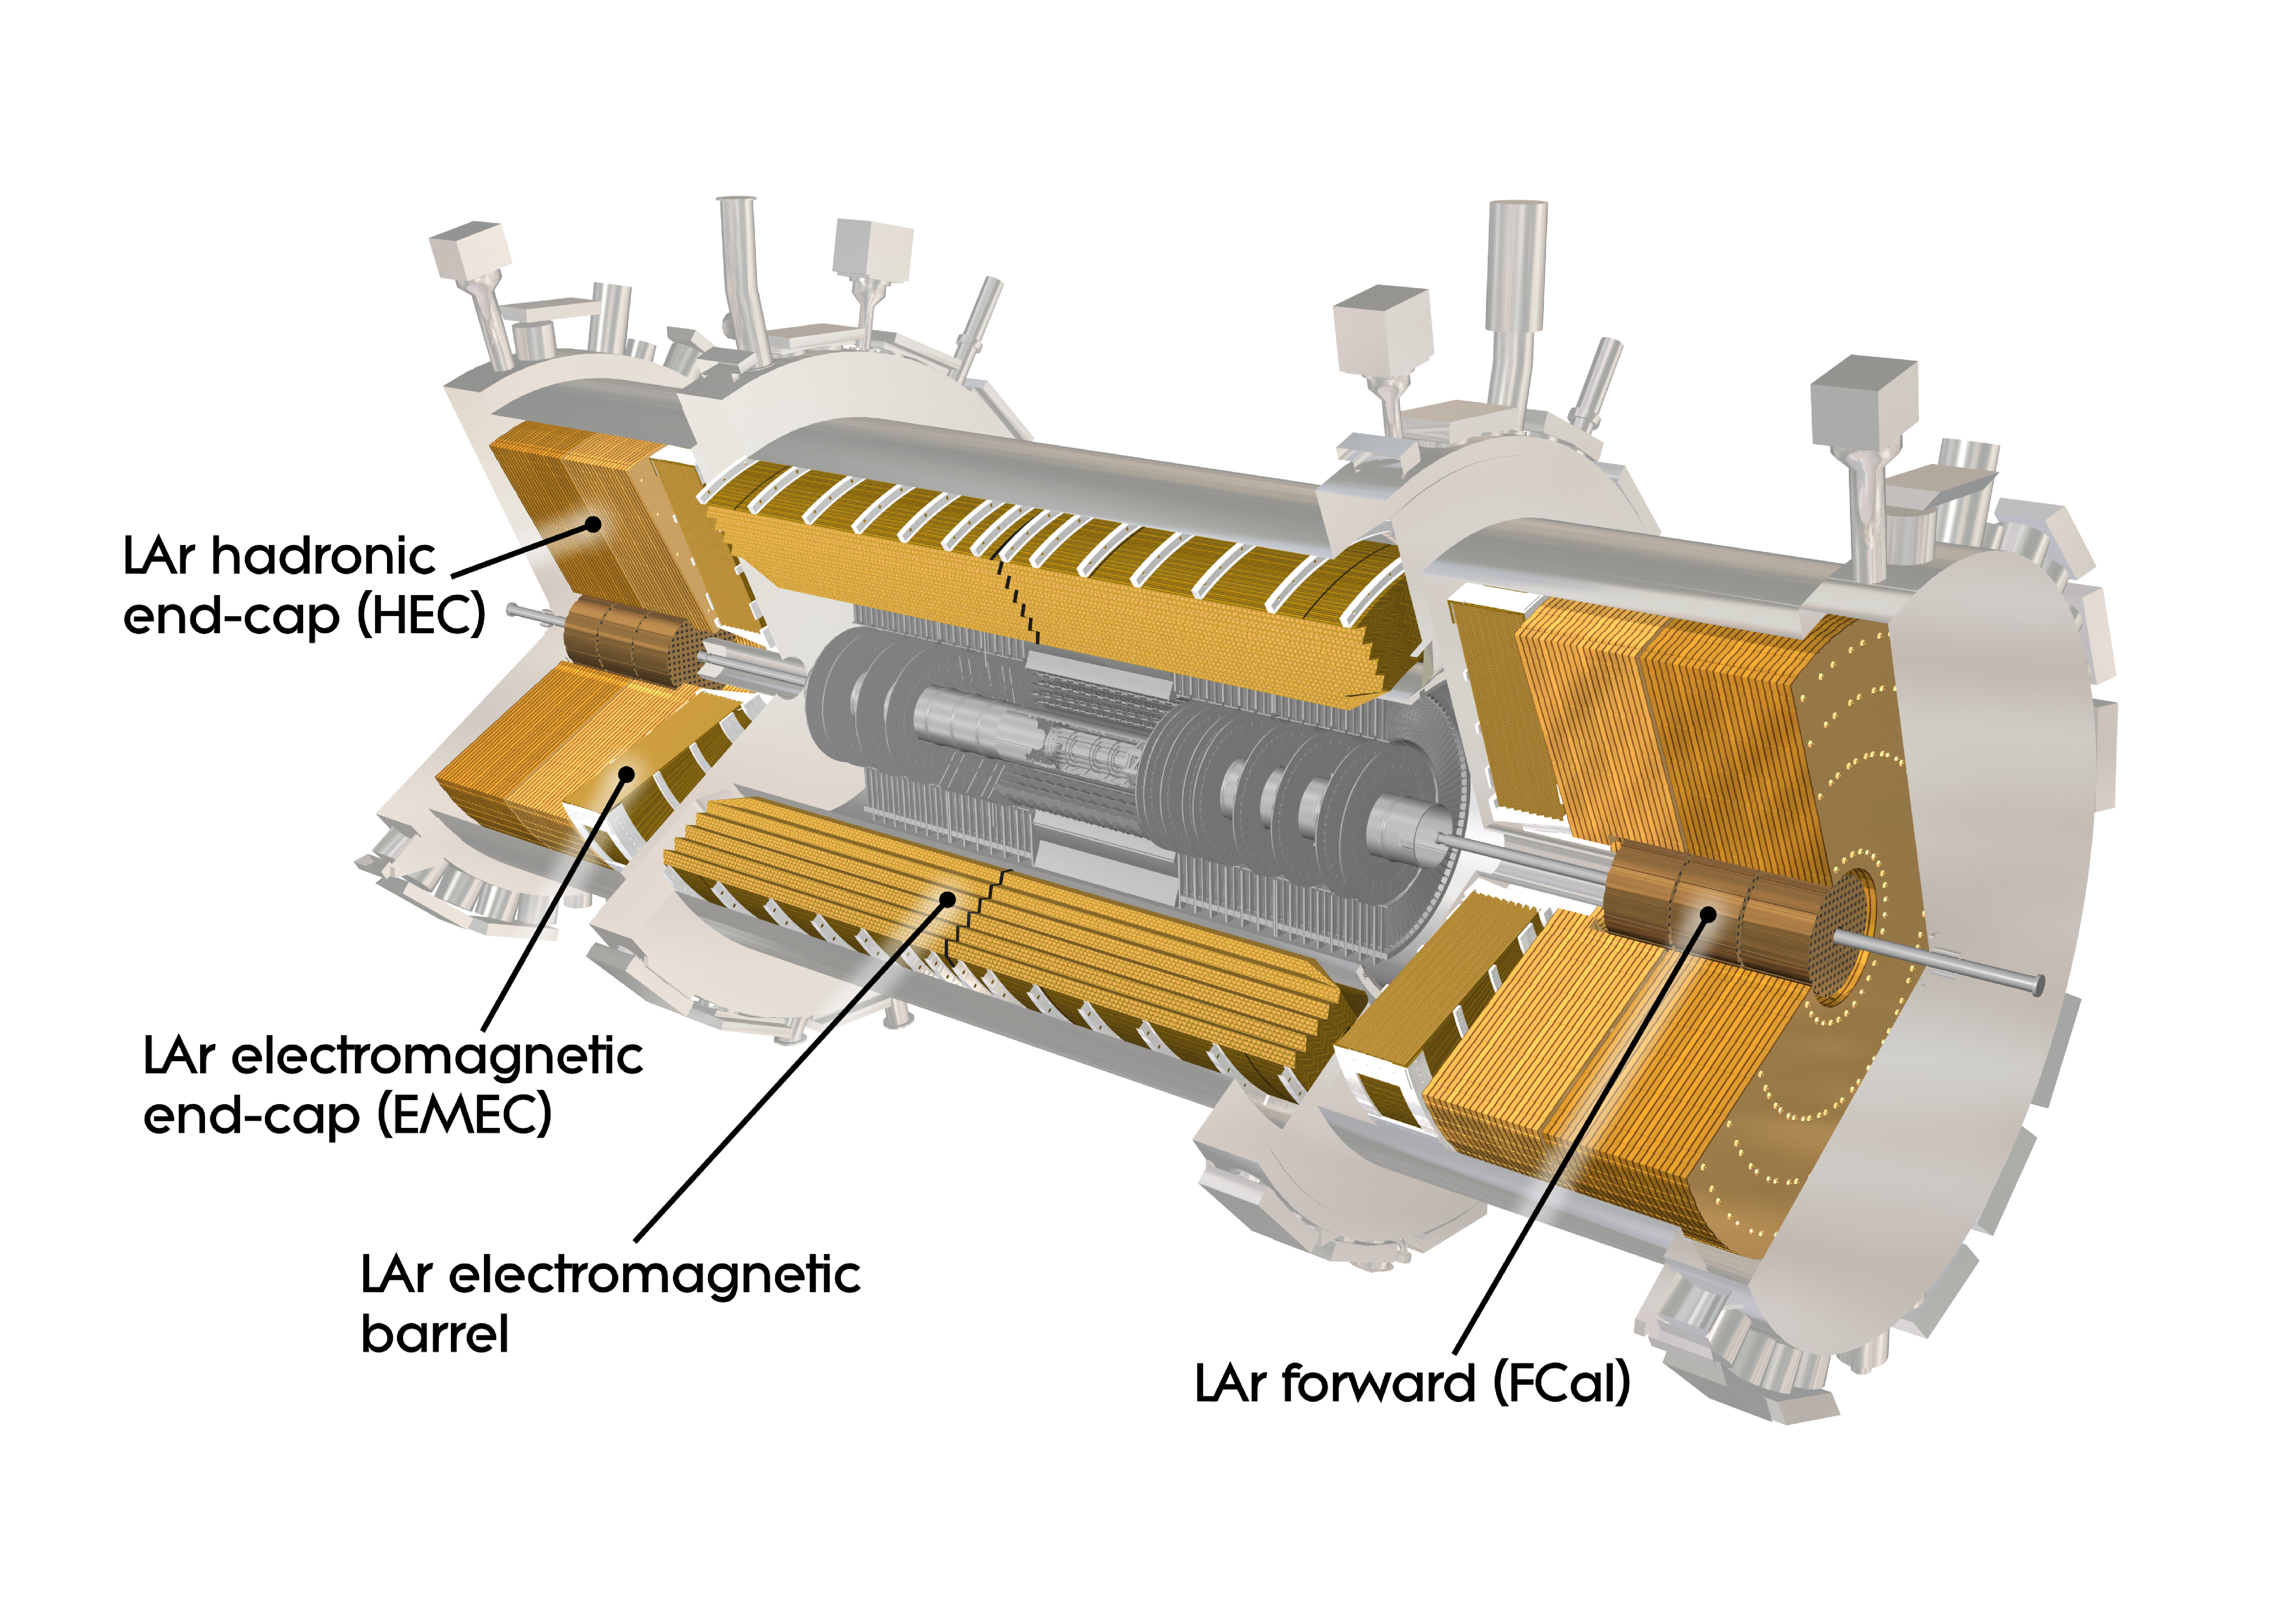
\includegraphics[width=0.70\textwidth]{ecal.eps}
% \caption{ECAL del detector ATLAS.}
% % \vspace{0.2cm}\footnotesize\textbf \sl{...}\vspace{0.2cm}
% \label{ecal}
% \end{figure}

El ECAL se divide en una parte central y los \textit{endcaps}. En la región de transición entre el \textit{barrel} y el \textit{endcap} se encuetra una zona no isntrumentada, por donde se conecta el detector. Esta región denominada \textit{crack}, está comprendida entre $1.37 < |\eta| < 1.52$. Es por este motivo que la mayoría de los análisis se requiere que los candidaos a fotones/electrones estén fuera de la región \textit{crack}.

{\bf Calorímetro hadrónico }

El calorímetro hadrónico cubre el rango $|\eta|< 4.9$ usando diferentes materiales. La parte del \textit{barrel} de este sistema utiliza acero como absorbente y tejas centelladoras como material activo. Las tejas están ubicadas radialmente y apiladas en profundidad. En la región de \textit{endcaps}, el calorímetro hadrónico se compone de dos ruedas perpendiculares al tubo del haz, hechas con placas de cobre y tungsteno como material absorbente y argón líquido como material activo. Estos detectores extienden la aceptancia del calorímetro de ATLAS hasta cubrir prácticamente la totalidad de ángulo sólido del punto de colisión.

\subsection{Espectrómetro de muones}

Los muones de alto $p_{T}$ generados en el punto de interacción tienen un altísimo poder de penetración y son poco interactuantes. Por ello el espectrómetro de muones se encuentra situado en la parte más exterior del detector ATLAS, alrededor del sistema de imanes de toroides, y está diseñado para obtener mediciones de alta precisión de posición e impulso de muones de alto $p_{T}$ . Este es el subdetector más grande y el que le da a ATLAS su tamaño característico (ver figura \ref{muon}. 

\begin{figure}
\centering
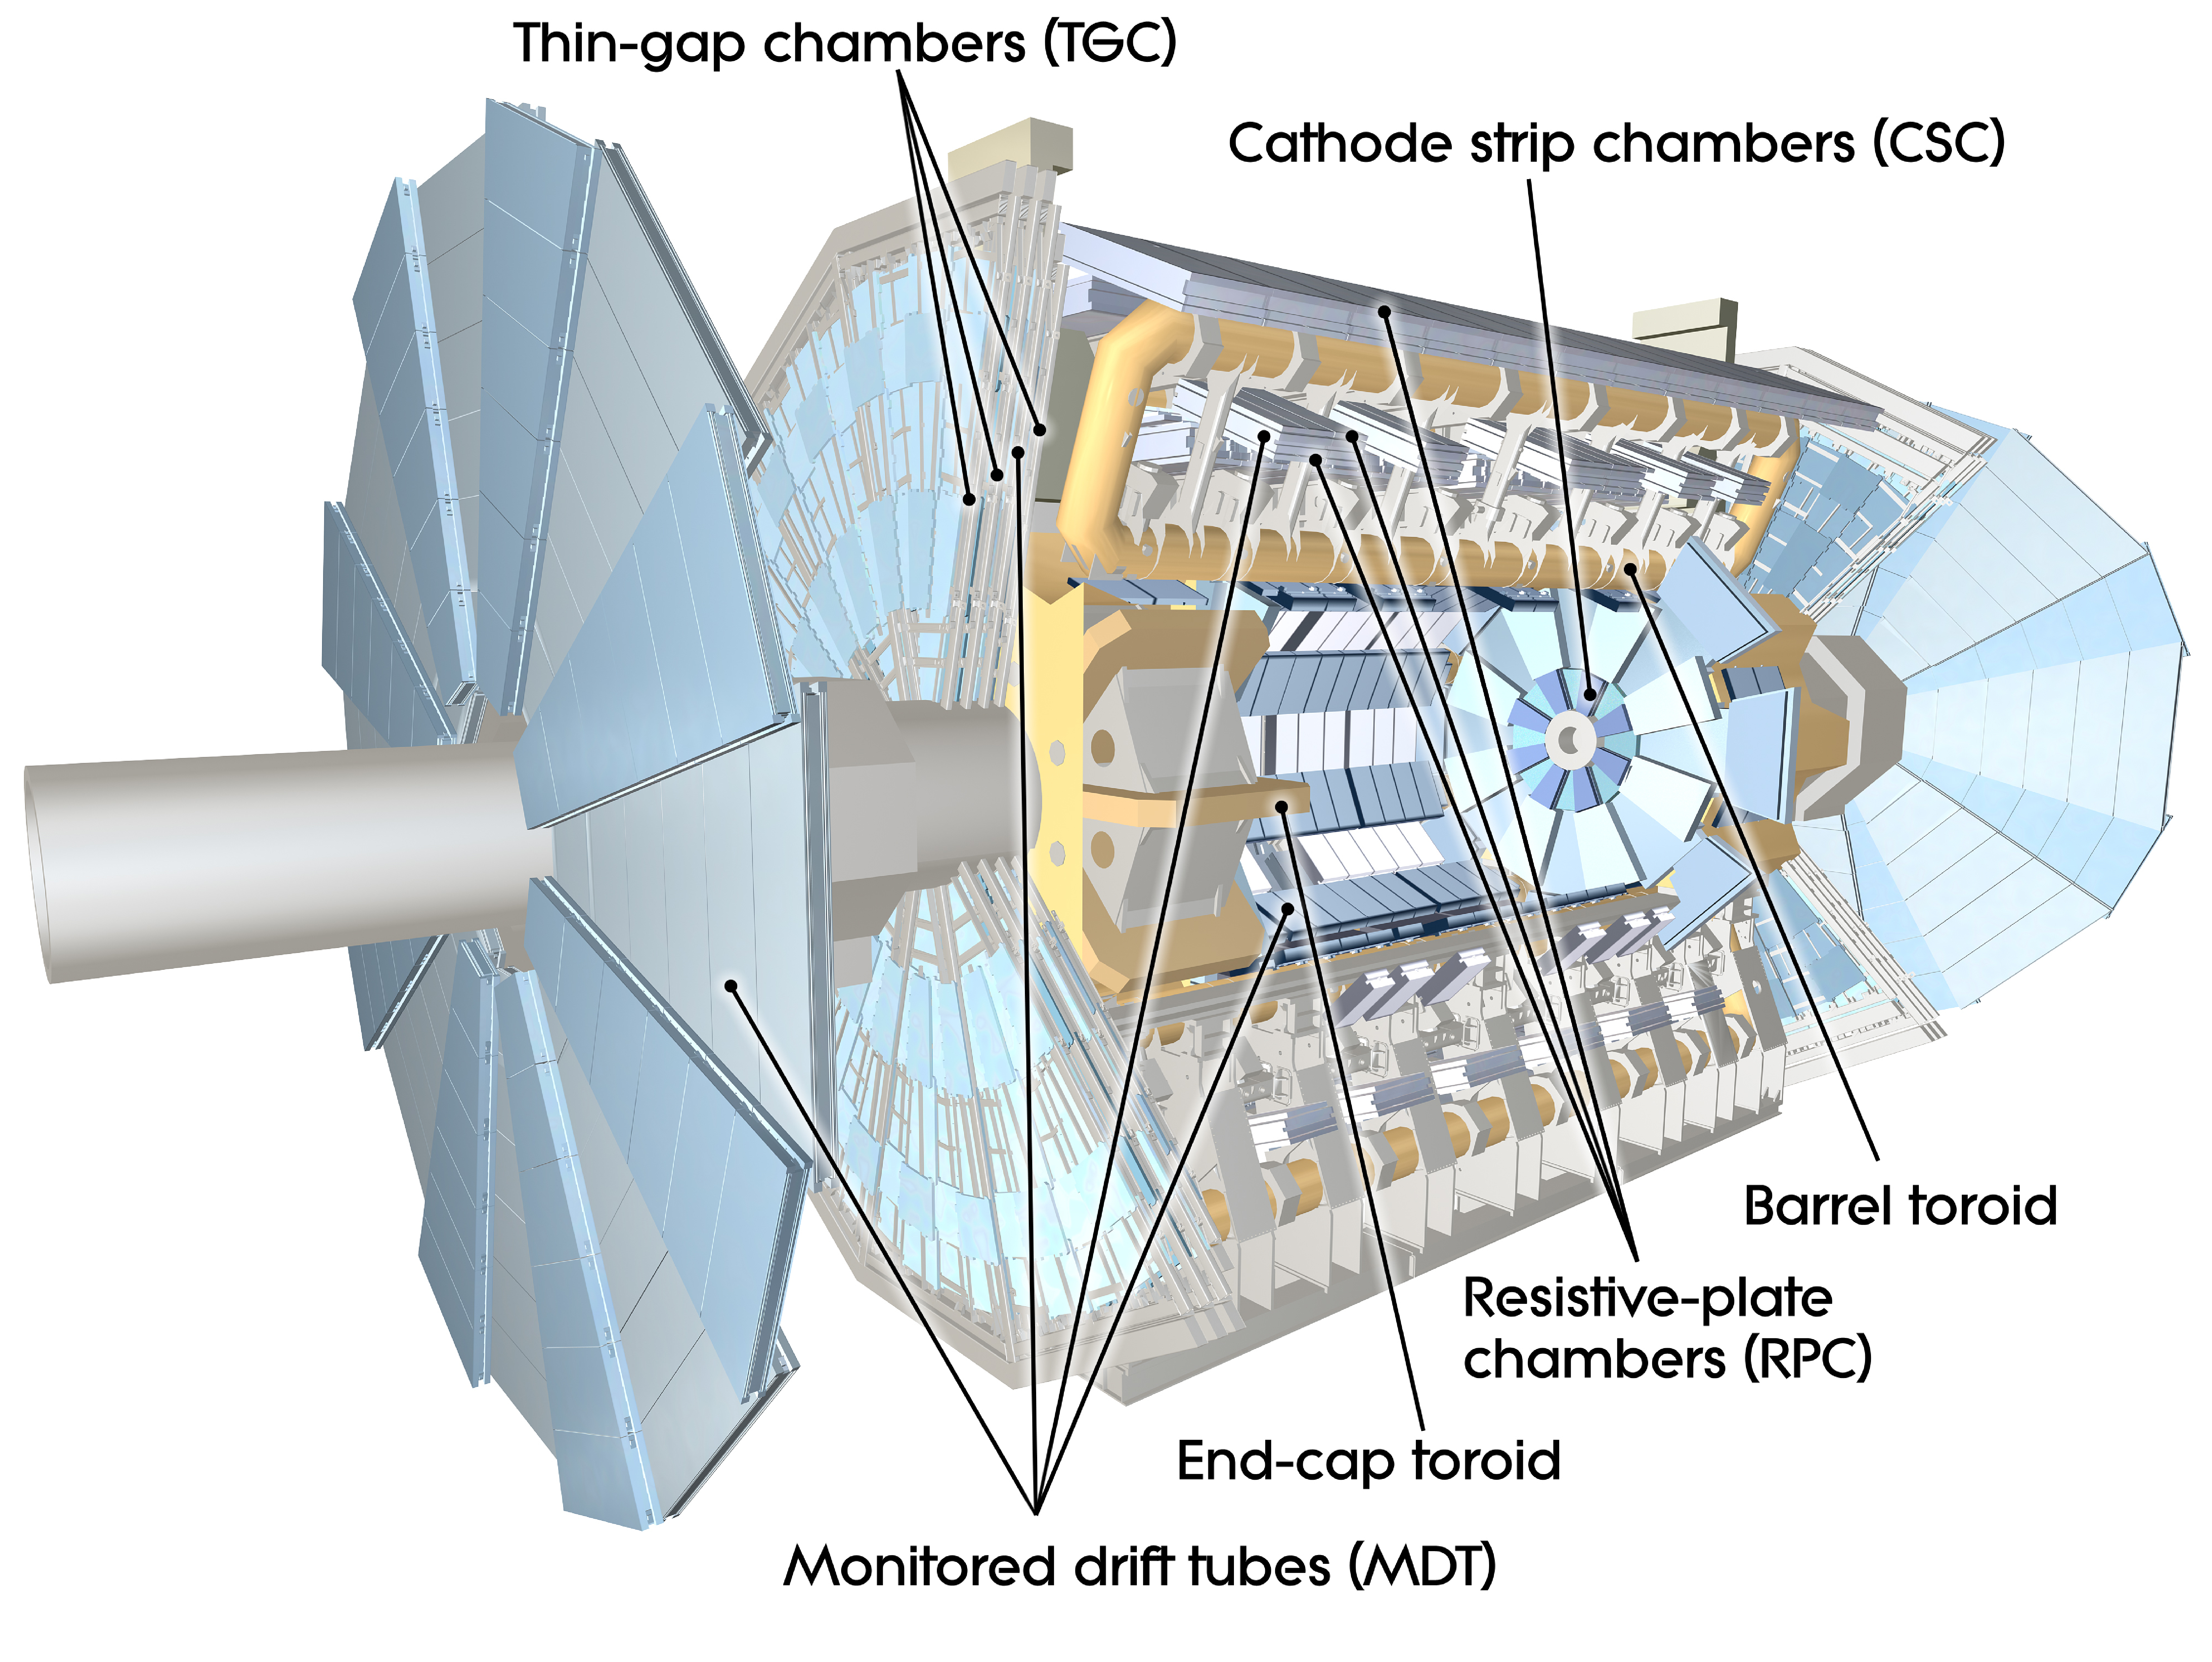
\includegraphics[width=0.60\textwidth]{muon.eps}
\caption{Espectrómetro de muones del detector ATLAS.}
% \vspace{0.2cm}\footnotesize\textbf \sl{...}\vspace{0.2cm}
\label{muon}
\end{figure}

Los muones al ser altamente penetrantes, son las únicas partículas (excepto las invisibles que no interactúan) que llegan al sistema de muones. Estos pierden parte de su energía mientras penetran las capas internas de ATLAS antes de llegar al espectrómetro de muones. La pérdida de energía es tenida en cuenta utilizando los depósitos de energía en los distintos calorímetros.

EXPLICAR FUNCIONAMIENTO DEL DETECTOR

\section{Sistema de \textit{trigger}}

El diseño del LHC permite tener una frecuencia de cruces de haces de 40 MHz y alrededor de 23 interacciones por cruce, lo que da una tasa de interacción protón-protón del orden del GHz. Debido a que el almacenamiento y el poder de cómputo de los datos recolectados son limitados, y considerando que no todos los eventos son de interés, es necesario reducir el flujo de datos incidentes a una frecuencia de $\sim 400$ Hz \cite{PERF-2011-02}. El sistema de trigger, es el encargado de filtrar los eventos que son de interés, para su poseterior análisis. 

El sistema de trigger de ATLAS consiste en una selección de eventos basada en tres niveles: Level 1 (L1), Level 2 (L2) y el Event Filter (EF), siendo los dos últimos los que coforman el High Level Trigger (HLT). Cada nivel permite analizar los eventos con mayor detalle, aumentando la precisión de los criterios de selección y la complejidad de los algoritmos utilizados.

El primer nivel de trigger se encarga de la selección inicial, reduciendo la frecuencia de eventos que pasan al siguiente nivel a $\sim 75$ kHz. Debido al tamaño limitado de las memorias temporales donde se guardan los datos de cada subdetector y al considerable tiempo de vuelo de las partículas hasta el espectrómetro de muones, la decisión debe tomarse en una escala de tiempo muy limitada ($2.5$ $\mu$s). El L1 está basado en hardware y selecciona objetos de alto $p_{T}$ construidos a partir de la información de varios subdetectores. Ciertas celdas del ECAL y el HCAL se utilizan para enviar señales al L1 con información de los objetos. La posición de cada objeto encontrado define una <<región de interés>> (RoI) en un evento potencialmente interesante, que se extiende como un
cono desde el punto de interacción a lo largo del detector.Lo mismo en el detector de muones, que tiene diferentes cámaras que permiten obtener una estimación rápida del $p_{T}$ de los muones. El diseño del L1 le parmite tener una aceptancia en el rango de $|\eta|<2.5$ para electrones, fotones, muones y taus; hasta $|\eta|<3.2$ para jets y $|\eta|<4.9$ para el cálculo de la energia transversa perdida.

El segundo nivel del trigger (L2) se centra únicamente en las RoIs donde el L1 encontró actividad, combinando información de todos los subdetectores dentro de cada una ($\sim$ 2 \% de la cobertura total del detector). El L2 consiste de una serie de algoritmos de reconstrucción y selección especializados, diseñados para reducir la frecuencia de eventos hasta aproximadamente 1 kHz. Estos algoritmos están implementados en clusters de procesamiento dedicados que analizan cada evento dentro de un tiempo de latencia medio de $\sim$40 ms. El menor flujo de información en este nivel del trigger permite calcular las variables calorimétricas con mayor precisión y hacer uso de la información de las trazas reconstruidas, haciendo posible la distinción entre fotones y electrones, y el rechazo de fondo proveniente en su mayoría de jets.

La última etapa de la selección del trigger se lleva a cabo en el Event Filter, que reduce la frecuencia de eventos a $\sim$400 Hz. En este nivel se tiene acceso a toda la  nformación del evento en los distintos subdetectores de ATLAS, con la máxima granularidad e incluyendo detalles sobre la calibración de energía de los calorímetros, la alineación de los subdetectores y el mapa de campo magnético. El tiempo de latencia relativamente largo disponible para tomar la decisión final sobre el evento ($\sim$4s) permite la reconstrucción completa del mismo, y el refinamiento de las variables y criterios de selección al nivel de aquellos implementados en el análisis offline. Los eventos aceptados por el EF son finalmente grabados a disco y distribuidos, accesibles offline para todos los análisis subsecuentes.

Para cada item del trigger se puede asignar además un factor de escala o prescale (PS), que define la frecuencia con la que un dado item es evaluado por el trigger (es decir solo en uno de cada PS eventos). Se habla de una cadena de trigger unprescaled si su factor de escala es PS = 1 en cada nivel, es decir, es evaluada en todos los eventos. La asignación de estos factores se hace incluso dinámicamente durante una toma de datos, para tener en cuenta el descenso de la luminosidad instantánea con el tiempo y mantener la tasa de procesamiento aproximadamente constante.


\chapter{Reconstrucción e identificación de objetos físicos}
% \addcontentsline{toc}{chapter}{Reconstrucción e identificación de objetos físicos}
\chaptermark{Reconstrucción e identificación de objetos físicos}

En el presente capítulo se describe la reconstrucción e identificación de electrones y fotones ya que son los objetos físicos principales utilizados en los estudios de esta Tesis. La reconstrucción de fotones y electrones en ATLAS se basa en las deposiciones locales de energía halladas en el ECAL, y la distinción entre unos y otros se   realiza mediante la información de las trazas reconstruidas en el ID. A su vez se aplican una serie de criterios de identificación y aislamiento, que permiten discriminarlos de falsos candidatos, o de procesos secundarios que los producen.

\section{Reconstrucción de electrones y fotones}

La  reconstrucción de fotones y electrones en ATLAS se basa en un algoritmo de clusterización \cite{Lampl:1099735} que busca deposiciones locales de energía en el calorímetro dentro de una ventana rectangular en el espacio ($\eta$, $\phi$) de tamaño fijo (\textit{Sliding Window clusterization}, SW) \cite{Monticelli:2227992}. La posición de la ventana se ajusta maximizando la energía transversa de todas las celdas contenidas. El tamaño óptimo de la ventana depende del tipo de partícula (más ancha para los electrones) a reconstruir y de la región del calorímetro (mas ancha en la región endcap). 

Aquellos \textit{clusters} electromagnéticos asociados con una traza reconstruida con $p_{T} > 0.5 \egev$, son clasificados como electrones. La definición para fotones es un poco más complicada ya que estos pueden convertir en un par $e^{+}e^{-}$ en el sector anterior al calorímetro. Los fotones convertidos están caracterizados por la presencia de al menos una traza asociada proveniente de un vértice reconstruido en el ID. La probabilidad de conversión varía entre un 40\% y un 80\% dependiendo de $\eta$, aunque solo aquellas que ocurren antes del TRT son eficientemente reconstruidas. 

Si no hay ninguna traza asociada a un dado \textit{cluster}, este es clasificado como un fotón no convertido. Aquellos \textit{clusters} asociados con trazas, que provienen de un vértice reconstruido en el ID, es clasificado como un fotón convertido. Además, para incrementar la eficiencia de reconstrucción de estos últimos, se consideran también aquellos casos donde solo una traza fue reconstruida, siempre que esta no posea ningún impacto en el B-Layer.

\section{Identificación de electrones y fotones}

La identificación de fotones se lleva a cabo mediante una serie de cortes rectangulares en un conjunto de variables que describen la forma y la estructura de las lluvias electromagnéticas según se propagan en el detector. Estas variables incluyen información de los calorímetros y, para el caso de fotones convertidos, del detector de trazas. Se definen dos conjuntos de cortes dependiendo de la rigurosidad de los mismos: \textit{loose} y \textit{tight}. Los cortes de cada conjunto han sido optimizados para asegurar una alta eficiencia de identificación de electrones/fotones aislados y de rechazo de fondo. 

Para la identificación de electrones se utiliza un algoritmo de identificación basado en el método de \textit{likelihood} (LH). El mismo consiste en una técnica de análisis multivariable que evalúa simultáneamente distintas propiedades de los candidatos a la hora de realizar la selección. El LH utiliza las funciones de densidad de probabilidad (PDFs) de la señal y del fondo de las distintas variables que describen a la lluvia electromagnética. Basada en esas PDFs, se calcula una probabilidad total del objeto de ser señal o fondo. Adicionalmente se utilizan variables discriminantes que se basan en la cantidad de impactos en el detector de trazas. Se utilizan tres cortes de discriminación: \textit{loose}, \textit{medium} y \textit{tight}. Los mismos se definen de tal forma de que los objetos seleccionado por uno sean un subconjunto de los otros. Es decir, los seleccionados por \textit{medium} son seleccionados también por \textit{loose}, y los seleccionados por \textit{tight} son seleccionados también por \textit{medium}.


La definición de algunas variables que determinan los distintos cortes se detallan a continuación. La definición de los cortes se muestra en la Tabla \ref{lmttable}.


\begin{itemize}

	\item \textbf{Fuga hadrónica}

		Es la energía transversa depositada en el calorímetro hadrónico, normalizada a la energía transversa del cluster electromagnético.

		\begin{equation}
		R_{\text{had}_{(1)}}=\frac{E_{T}^{\text{had}}}{E_{T}}
		\end{equation}

		En la región de transición barrel-endcap del HCAL, se utiliza el depósito de energía en todo el calorímetro hadrónico para minimizar los efectos de la degradación de resolución ($R_{\text{had}}$). En el resto del detector, se mide sólo la energía hadrónica depositada en la primera capa del HCAL ($R_{\text{had}_{(1)}}$).

	\item  \textbf{Perfil lateral de energía en $\eta$ (2$^{\text{da}}$ capa del ECAL)}

		\begin{equation}
		R_{\eta}=\frac{E_{3\times 7}^{S2}}{E_{7\times 7}^{S2}}
		\end{equation}

 		donde $E_{i\times j}^{S2}$ es la suma de las celdas en la segunda capa del calorímetro electromagnético contenidas en una ventana $i\times j$ (en $\Delta \eta \times \Delta \phi$).

	\item  \textbf{Perfil lateral de energía en $\phi$ (2$^{\text{da}}$ capa del ECAL)}

		\begin{equation}
		R_{\phi}=\frac{E_{3\times 3}^{S2}}{E_{3\times 7}^{S2}}
		\end{equation}

 		donde $E_{i\times j}^{S2}$ es la suma de las celdas en la segunda capa del calorímetro electromagnético contenidas en una ventana $i\times j$ (en $\Delta \eta \times \Delta \phi$).

	\item  \textbf{RMS del perfil lateral de energía en $\eta$ (2$^{\text{da}}$ capa del ECAL)}


		\begin{equation}
		w_{\eta_{2}}=\sqrt{\frac{\sum E_{i}\eta_{i}^{2}}{\sum E_{i}}- \left(\frac{\sum E_{i}\eta_{i}}{\sum E_{i}}\right)^{2}}
		\end{equation}

		mide el ancho lateral de las lluvias electromagnéticas, donde $E_{i}$ es la energía de la i-ésima celda del calorímetro electromagnético contenida en una ventana de $3\times 5$ celdas en $\eta \times \phi$.

	\item  \textbf{Perfil lateral de energía en $\eta$ (1$^{\text{ra}}$ capa del ECAL)}

		\begin{equation}
		F_{\text{side}}=\frac{E(\pm 3)-E(\pm 1)}{E(\pm 1)}
		\end{equation}

		mide la contención lateral de la cascada electromagnética a lo largo de $\eta$. $E(\pm n)$ es la energía en las $\pm n$ celdas alrededor de aquella con la deposición máxima.

	\item  \textbf{RMS del perfil lateral de energía en $\eta$ (3 \textit{strips}, 1$^{\text{ra}}$ capa del ECAL)}

		\begin{equation}
		w_{s,3}=\sqrt{\frac{\sum E_{i}(i-i_{\text{max}})^{2}}{\sum E_{i}}}
		\end{equation}

		mide el ancho de la lluvia electromagnética a lo largo de $\eta$ en la primera capa del calorímetro electromagnético usando solo la banda con mayor deposición de energía ($i_{\text{max}}$) y sus vecinas inmediatas.

	\item  \textbf{RMS del perfil lateral de energía en $\eta$ (total, 1$^{\text{ra}}$ capa del ECAL)}

		$w_{s,\text{tot}}$ está definida de la misma forma que $w_{s,3}$, pero utiliza todas las bandas de la primera capa del calorímetro electromagnético en una ventana $\Delta\eta\times\Delta\phi = 0.0625 \times 0.2$, que corresponde aproximadamente a $20\times 2$ bandas en $\eta \times \phi$.

	\item  \textbf{Diferencia al segundo máximo}

		\begin{equation}
		\Delta E=[E_{2^{nd} \:\text{max}}^{S1} - E_{\text{min}}^{S1}]
		\end{equation}

		es la diferencia entre la energía de la banda con la segunda energía más grande $E_{2^{nd} \:\text{max}}^{S1}$ , y la mínima energía $E_{\text{min}}^{S1}$ entre la anterior y la celda con la máxima deposición. En caso de no haber segundo máximo se fija $\Delta E = 0$.

	\item  \textbf{Asimetría de los dos máximos locales en $\eta$}

		\begin{equation}
		\Delta E_{\text{ratio}}=\frac{E_{1^{st} \:\text{max}}^{S1} - E_{2^{nd} \:\text{max}}^{S1}}{E_{1^{st} \:\text{max}}^{S1} + E_{2^{nd} \:\text{max}}^{S1}}
		\end{equation}
 
 		mide la diferencia relativa entre las energías de las dos celdas con máxima deposición. En caso de no haber segundo máximo se fija $E_{\text{ratio}} = 1$.


\end{itemize}

\renewcommand{\arraystretch}{1.0}
\begin{table}	
\centering
\caption{Detalle de las diferentes variables usadas para la selección \textit{loose} (L) y \textit{tight} (T) de fotones y electrones. El $\checkmark$ indica cuándo la selección requiere de esa variable\cite{ATLAS:2016iqc} \cite{Tripiana:1433788}.}
 \makebox[0.5\textwidth][c]{
 \begin{tabular}{ r p{8cm} c | c c | c }

	\hline

	\multirow{2}{*}{Categoría} & \multirow{2}{*}{Descripción} & \multirow{2}{*}{Nombre} & \multicolumn{2}{ c |}{$\gamma$} & \multirow{2}{*}{$e$} \\

		&	&	& L & T &   \\

	\hline

	Aceptancia & $|\eta| < 2.37$, excluyendo $1.37 < |\eta| < 1.52$  & - & $\times$ & $\checkmark$ & $\times$  \\

	Fuga hadrónica & Cociente entre $E_{T}$ en la primera capa del calorímetro hadrónico y $E_{T}$ del \textit{cluster} electromagnético & $R_{\text{had}_{1}}$ & $\checkmark$ & $\checkmark$ & $\checkmark$ \\

		& Cociente entre $E_{T}$ en todo el calorímetro hadrónico y $E_{T}$ del \textit{cluster} electromagnético $(|\eta| \le 0.8$ y $|\eta| \ge 1.37)$ & $R_{\text{had}}$ & $\checkmark$ & $\checkmark$ & $\checkmark$  \\

	ECAL (3$^{ra}$ capa) & Fracción de energía en la tercer capa del ECAL & $f_{3}$ & $\times$ & $\times$ & $\checkmark$  \\
	

	ECAL (2$^{da}$ capa) & Ancho lateral de la lluvia en dirección de $\eta$ & $w_{\eta_{2}}$ & $\checkmark$ & $\checkmark$ & $\checkmark$ \\

		& Cociente entre la suma de las energías de las 3 $\times$ 7 celdas y la suma de 5 $\times$ 7 celdas, ambas en torno al centro del \textit{cluster} & $R_{\eta}$ & $\checkmark$ & $\checkmark$ & $\checkmark$ \\

		& Cociente entre la suma de las energías de las 3 $\times$ 3 celdas y la suma de 3 $\times$ 7 celdas, ambas en torno al centro del \textit{cluster} & $R_{\phi}$ & $\times$ & $\checkmark$ & $\checkmark$ \\

	ECAL (1$^{ra}$ capa) & Ancho lateral de la lluvia en 3 \textit{strips} alrededor del máximo & $w_{s,3}$ & $\times$ & $\checkmark$ & $\times$ \\

		& Ancho lateral total de la lluvia & $w_{s,\text{tot}}$ & $\times$ & $\checkmark$ & $\checkmark$ \\

		& Fracción de energía fuera de las 3 \textit{strips} centrales pero dentro de las 7 & $F_{\text{side}}$ & $\times$ & $\checkmark$ & $\times$ \\

		& Diferencia entre la energía de la \textit{strip} con el segundo mayor depósito y la menor energía entre los dos primeros máximos locales & $\Delta E$ & $\times$ & $\checkmark$ & $\times$ \\

		& Asimetría entre el primer y segundo máximo & $E_{\text{ratio}}$ & $\times$ & $\checkmark$ & $\checkmark$  \\

		& Fracción de energía en la primera capa del ECAL & $f_{1}$ & $\times$ & $\times$ & $\checkmark$  \\

	ID & Parámetro de impacto transverso& $d_{0}$ & $\times$ & $\times$ & $\checkmark$ \\

		& Momento perdido en la traza entre el primer punto de detección y el último, dividido el momento total original & $\Delta p/p$ & $\times$ & $\times$ & $\checkmark$  \\

	TRT & Probabilidad \textit{likelihood} basa en la radiación de transición en el TRT & eProbabilityHT & $\times$ & $\times$ & $\checkmark$  \\

	ECAL+ID & $\Delta\eta$ entre la traza extrapolada al calorímetro y el \textit{cluster} en la primer capa& $\Delta\eta_{1}$ & $\times$ & $\times$ & $\checkmark$ \\

	\hline

\end{tabular}}
\label{lmttable}
\end{table}
\renewcommand{\arraystretch}{1}

Por último un algoritmo adicional es aplicado para resolver ambigüedades residuales en candidatos a fotones que son también reconstruidos como electrones. Diferentes estrategias son utilizadas dependiendo del estado de conversión de los fotones según es explica en la Referencia \cite{ambiguity}.


\section{Criterios de aislamiento}

Luego de realizar la identificación, es necesario distinguir entre electrones y fotones directos (aquellos producidos en la colisión), mal reconstruidos o de los no directos producidos de decaimientos de hadrones ($\pi^{0}$, $\eta$, etc.) dentro de jets.

Los fotones o electrones provenientes por ejemplo, del punto de interacción, o los electrones provenientes de $Z\rightarrow ee$, poseen baja actividad hadrónica en su vecindad. En cambio en los no directos, se espera que haya un gran actividad provenientes de los objetos que acompañan al jet dentro del que fueron producidos o erróneamente identificados. Para realizar esta distinción se utiliza un criterio de aislamiento que se basa en medidas calorimétricas o en las trazas reconstruidas en el entorno del objeto.

El aislamiento de trazas se define a partir de considerar un cono de radio $R=\sqrt{\Delta\eta^{2}+\Delta\phi^{2}}$ centrado en el baricentro del \textit{cluster} electromagnético asociado al objeto. A todas las trazas dentro de este cono se le pueden aplicar ciertos cortes, como $p_{T}>1 \egev$, impactos en el SCT, etc. Además, se requiere que aquellas trazas en un cono interno con $R=0.1$, no provengan de un vértice de conversión, a fin de remover los fotones convertidos. El aislamiento de trazas ha mostrado ser altamente eficiente tanto para retener señal como para rechazar falsos candidatos del fondo, aún luego de la selección descripta en la sección anterior. Aun así, el criterio más utilizado es el aislamiento calorimétrico.

El aislamiento calorimétrico, $E_{T}^{\text{iso}}$, es calculado a partir de las celdas en ambos calorímetros (ECAL y HCAL). Nuevamente se define un cono con un cierto radio $R$ centrado en el baricentro del \textit{cluster} del objeto, y la suma de la energías de todas las celdas contenidas en ese cono se denomina $E_{T}^{\text{iso}}$. 

A fin de remover la contribución energética de la lluvia electromagnética desarrollada por el propio objeto al cono de aislamiento, el núcleo central de $N_{\eta}\times N_{\phi} = 5 \times 7$ celdas en el segundo compartimiento del ECAL, es ignorado en la suma, como se esquematiza en la Figura \ref{isolation}. Se considera que dentro de esta región ignorada, se concentra el 95\% de la energía de la lluvia electromagnética, por lo que solo el 5\% de la energía del objeto contribuye a esta región. Por otro lado, todas las celdas contenidas dentro del cono en el HCAL son consideradas para la suma, ya que se espera que el ECAL contenga toda lluvia electromagnética desencadenada por el objeto inicial. 

Para fotones, el valor típico de $R$ es $0.4$, y el corte de aislamiento es $E_{T}^{\text{iso}}<2.45 \egev + 0.022 \times p_{T}$ (donde el $p_{T}$ corresponde al momento transverso del objeto reconstruido e identificado). En cambio los electrones pasan por un criterio que tiene dependencia en $\eta$ y $p_{T}$ denominado \textit{Gradient Loose}, con requerimientos tanto en las variables calorimétricas como en las asociadas a la traza \cite{ATL-PHYS-PUB-2015-037_extra}.


% En cambio en los electrones pasan por un criterio denominando \textit{Gradient Loose}, en el cual el valor de $R$ depende del $p_{T}$ de los mismos. En este caso para el aislamiento calorimétrico $R=0.2$ y para el aislamiento de trazas $R=10\egev/p_{T}$

\begin{figure}
\centering
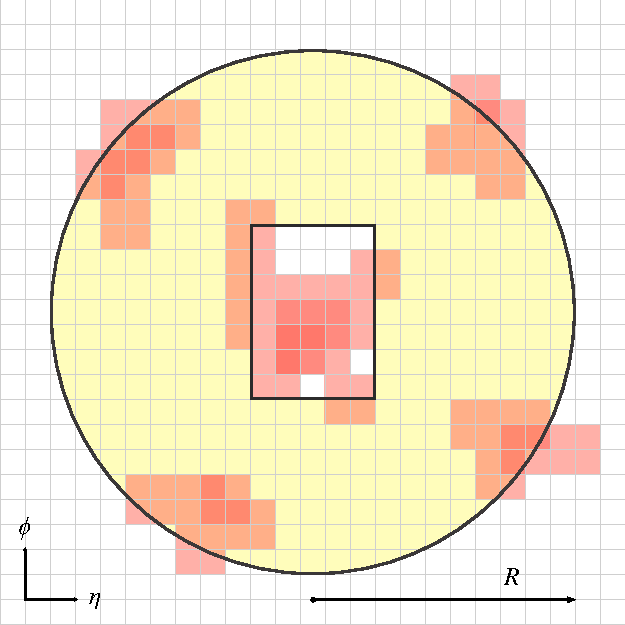
\includegraphics[width=0.50\textwidth]{iso.pdf}
\caption{Esquema ilustrando el cálculo de la energía de aislamiento del fotón. La \textit{grid} representa la granularidad de las celdas del calorímetro electromagnético. El cono de color amarillo de radio $R$ rodea al candidato. La energía del candidato a fotón o electrón está mayormente contenida en el rectángulo central de $5 \times 7$ en $\Delta\eta \times \Delta\phi$.}
\label{isolation}
\end{figure}

\section{Energía faltante}

Una variable de suma importancia en la búsqueda de partículas supersimétricas, es la energía transversa faltante ($\met$). Como se mencionó anteriormente, el momento transverso se debe conservar en todo el proceso, y cualquier desequilibrio en el mismo se lo asocia a $\met$. Puede indicar la presencia de partículas indetectables como neutrinos o nuevas partículas estables, o que interactúan débilmente con la materia.

El momento transverso faltante ($p_{T}^{\text{miss}}$) se define como el valor negativo de la suma del momento transverso de todas las partículas detectadas, y su magnitud es lo que se denomina energía transversa faltante. Esta es calculada con un algoritmo basado en objetos \cite{Khoo:2012749}. El algoritmo utiliza los objetos físicos construidos y calibrados descriptos en las secciones anteriores. Los depósitos de energía en el calorímetro (topo-clusters) son asociados a los objetos de alto $p_{T}$ en el siguiente orden: electrones, fotones, jets y muones. Los depósitos que no están asociados a ningún objeto son incluidos en el término \textit{soft}. El momento transverso es calculado entonces como:

\begin{equation}
p_{T}^{\text{miss}}=\left(p_{T}^{\text{miss}}\right)^{e} + \left(p_{T}^{\text{miss}}\right)^{\gamma} + \left(p_{T}^{\text{miss}}\right)^{\text{jet}} +\left(p_{T}^{\text{miss}}\right)^{\mu} + \left(p_{T}^{\text{miss}}\right)^{\text{soft}}
\end{equation}

\noindent
donde cada término es calculado como el negativo de la suma de los objetos reconstruidos y calibrados, más el término \textit{soft}. La contribución de los taus, se incluye en el término de jets o en el \textit{soft}, debido a que los mismos decaen hadrónicamente. Finalmente la energía transversa faltante se define como:

\begin{equation}
\met=|p_{T}^{\text{miss}}|
\end{equation}



\clearpage

\chapter{Estrategia general del análisis}
% \addcontentsline{toc}{chapter}{Estrategia general del análisis}
\chaptermark{Estrategia general del análisis}


El análisis para el cual está orientada esta tesis, consiste en la búsqueda de Supersimetría en eventos con un fotón aislado muy energético, jets y gran cantidad de energía faltante. La estrategia general consiste en el conteo del número de eventos observado en una cierta región del espacio de observables, rica en eventos de la señal considerada.

Para un correcto procedimiento, es necesario es conocer los procesos del SM que tengan como estado final uno equivalente a de la señal buscada, que toman el rol de fondo en el análisis. En este caso van a ser los que tienen un fotón, jets y energía faltante en el estado final. Estos pueden dividirse en varias categorías. Por un lado, los procesos que dan lugar a eventos con un fotón y energía faltante
real, es decir, los que llamamos fondos irreducibles. Estos son:

\begin{itemize}

	\item $Z(\rightarrow \nu\nu)$ + $\gamma$

	\item $W (\rightarrow l\nu)$ + $\gamma$

	\item $t \overline{t}$ + $\gamma$

\end{itemize}

También es posible que, aunque el proceso no tenga fotones en el estado final, un electrón o un jet sean identificados como un fotón, dando lugar a un estado final idéntico al buscado. En esta categoría están:

\begin{itemize}

	\item $W (\rightarrow l\nu)$ + jets

	\item $Z (\rightarrow \nu\nu)$ + jets

	\item $t \overline{t}$

	\item WW, ZZ, WZ

\end{itemize}

Y por último, también puede haber procesos que a pesar de no generar energía faltante real, poseen lo que se denomina energía faltante instrumental, proveniente generalmente de la incorrecta reconstrucción de la energía de los jets. De esta manera, pueden dar lugar a eventos con el estado final de interés, los procesos QCD:

\begin{itemize}

	\item $\gamma$+jets

	\item multijet, con alguno de los jets identificado como fotón

	\item $Z(\rightarrow ll)$ + $jets$, donde un leptón o un jet es identificado como un fotón

\end{itemize}



\section{Regiones de señal, control y validación}

Al estudiar fenómenos de nueva física es necesario definir una región en el espacio de observables, donde el modelo de señal predice un exceso significativo de eventos sobre el nivel de fondo. Esta región se llama region de señal (SR). El análisis consiste basicamente en estimar las contribuciones de los procesos del SM que contaminan eta región. Para esto existen dos técnicas principales: utilizar directamente simulaciones Monte Carlo, o utilizar métodos basados en los propios datos observados. En algunos casos se emplea un tercer método para estimar los fondos, que consiste en utilizar la estimación proveniente de las simulaciones MC, pero corregida a partir de los datos. Para esto se define una región de control (CR) en la cual el fondo dominante pueda ser controlado comparándolo con los
datos observados en esa misma región. 

Las CR son diseñadas especialmente para tener una alta pureza en uno de los procesos de fondo y deben estar libres de contaminación de señal. A través del ajuste a los datos, el número de eventos observado en una CR es usado para normalizar el número de eventos estimado de fondo en todas las regiones, especialmente en la SR. Otra componente importante del análisis es la validación del método utilizado para predecir losfondos en las SR. Con este objetivo se definen regiones de validación (VR) que se encuentren entre las CR y las SR en términos de los principales observables cinemáticos en los criterios de selección. El diseño de las VR comprende un compromiso entre minimizar la contaminación de la señal, y a su vez ser efectivas en la validación de la extrapolación entre CR y SR. 

\chapter{Electrones identificados como fotones}
% \addcontentsline{toc}{chapter}{Electrones identificados como fotones}
\chaptermark{Electrones identificados como fotones}

Existe un fondo que contribuye a procesos asociados a fotones y jets como estado final, donde un electrón del estado final es identificado como un fotón. Este puede provenir de procesos del SM, como los que producen bosones W y Z + jets, y $t \overline{t}$. El objetivo es estimar este fondo calculando un factor de identificación errónea en función de las variables $\eta$ y $p_{T}$ de los objetos.

\section{Medición del factor}

De una muestra de $Z\rightarrow ee$, se buscan eventos con un par electrón-positrón, o con un par electrón-fotón. Los requisitos para los electrones son $p_{T} > 25GeV$, identificados como \textit{medium} y punto de trabajo de aislamiento \textit{gradient loose}. Para los fotones los requisitos son $p_{T} > 25GeV$, \textit{tight} y aislados. A ambos se les solicita que tengan un $\eta_{BE}<2.37$, fuera de la region entre $1.37$ y $1.52$, con un parámetro de impacto $d_{0}$ con una significancia menor a 5, y con $|\Delta z_{0}sin\theta|<5$. Además, si un electrón y un fotón son reconstruidos con $\sqrt{\Delta\phi^{2}+\Delta\eta^{2}}<0.4$, el fotón es descartado del evento. Además, a todos los pares se les solicita que su masa invariante esté entre 75 y 105 GeV. Finalmente, en el caso de que existiese más de un par en el evento, se utiliza el que tiene la masa invariante más cercana a la del bosón Z.

Cuando el evento contiene un par electrón-eletrón, en un histograma con bines de $\eta$ y $p_{T}$ ($N^{ee}[\eta , p_{T}]$), se suma una entrada en el bin correspondiente al $\eta$ y $p_{T}$ de cada uno de los electrones. En el caso de que el evento tenga un par electrón-fotón, en otro histograma ($N^{eg}[\eta , p_{T}]$), se suma una entrada en el bin correspondiente al $\eta$ y $p_{T}$, solamente del fotón. El factor se obtiene como:

\begin{equation}
F_{e\rightarrow\gamma}[\eta , p_{T}]=\frac{N^{eg}[\eta , p_{T}]}{N^{ee}[\eta , p_{T}]}
\end{equation}

Cada entrada en los histogramas está pesada. El peso se obtiene clasificando a los pares según el tipo (\textit{ee}-\textit{eg}) y según la región donde se reconstruían los objetos (\textit{EE}-\textit{EB}-\textit{BB}). Para cada uno se calcula su masa invariante, y finalmente el peso resulta de la relación entre señal (S) y fondo (B): $w=\frac{S}{S+B}$. Esto se debe a que los pares tienen un probabildiad de no provenir del decaimiento del bosón Z, sino de otros procesos no resonantes de fondo. La relación entre señal y fondo tiene en cuenta esta probabiliadad.

La concepción del metodo proviene de la siguiente consideración. Sea $\epsilon_{i}$ la eficienca de reconstruir un electrón, con un $\eta$ y $p_{T}$ correspondientes al bin \textit{i} del histograma. Para una muestra de \textit{N} pares de electrones y positrones reales (dentro del rango de masa), decimos que $f_{ij}$ es la fracción de pares para los cuales el electrón \textit{leading} (\textit{sub-leading}) cae dentro del bin \textit{i} (\textit{j}). Considerando solamente electrones-positrones provenientes del decaimiento de un bosón Z, el número de eventos en el bin \textit{i} del histograma $N^{ee}[\eta , p_{T}]$ sería entonces:

\begin{equation}
N_{i}^{ee} = \sum_{i}\epsilon_{i}\epsilon_{j}f_{ij}N + \sum_{j}\epsilon_{j}\epsilon_{i}f_{ji}N = \epsilon_{i}N\sum_{j}\epsilon_{j}(f_{ij}+f_{ji})
\end{equation}

De forma análoga, ahora considerando que $p_{i}$ es la proporción de fotones reconstruídos como electrones en el bin \textit{i}, la cantidad de eventos en el bin \textit{i} del histrograma $N^{eg}[\eta , p_{T}]$ es:

\begin{equation}
N_{i}^{eg} = \sum_{i}p_{i}\epsilon_{j}f_{ij}N + \sum_{j}p_{j}\epsilon_{i}f_{ji}N = p_{i}N\sum_{j}\epsilon_{j}(f_{ij}+f_{ji})
\end{equation}

El factor que determina la proporción de electrones reconstruidos como fotones se define como:

\begin{equation}
F_{e\rightarrow\gamma}[\eta , p_{T}]\equiv\frac{N^{eg}}{N^{ee}}=\frac{p_{i}}{\epsilon_{i}}
\end{equation}

Por ende, no es la proporción de fotones mal reconstruidos, sino que es el cociente entre esa proporción y la eficiencia de recosntruir un electrón. De tal forma de que el fondo correspondiente a electrones identificados como fotones resulte:

\begin{equation}
N_{e\rightarrow\gamma}(\eta , p_{T} , ... )=F_{e\rightarrow\gamma}(\eta , p_{T})\cdot N_{e}(\eta , p_{T} , ...)
\end{equation}
	
Donde $N_{e}(\eta , p_{T} , ...)$ corresponde al número de electrones en el estado final.

Los datos utilizados para el análisis corresponden al Run 2 del LHC. Para los ajustes de la masas invariantes se utiliza como modelo de señal una \textit{double-sided Crystall-ball}. Para el fondo se utiliza ???. Los resultados de los ajustes obtenidos para cada clasificación de los pares se pueden observar en las figuras ...

Se consideran distintas fuentes de incetezas sistemáticas. Una de ellas proveniente de la variación tanto el rango del fit, como el rango de masa de aceptación de los pares. El rango noinal del fit es ??? y se varía ???. El rango nominal de la masa es ??? y se varía ???. También se utiliza una muestra de Monte-Carlo del proceso $Z\rightarrow ee$, calculando su "verdadero" factor y considerando esta discrepancia como sistemático. Se tuvo en cuenta también, como fuente de sistemático, la variación en los valores de los factores al utilizar otra función para el ajuste del fondo, utilizándose ???.

Los resultados obtenidos para el factor en bines de $\eta , p_{T}$ se muestran en la tabla...

% \chapter{Electrones identificados como fotones}\label{ch:e_fake}
\chaptermark{Electrones identificados como fotones}

Como ya se mencionó anteriormente, existe un fondo que contribuye a procesos asociados a fotones y jets como estado final, donde un electrón del estado final es identificado como un fotón. Este puede provenir de procesos del SM, como los que producen bosones W y Z + jets, y $t \overline{t}$. El mismo es difícil de estimar a partir de simulaciones, ya que dependen en gran medida de la estructura y material del detector que es muy compleja de modelar en todos sus detalles. El objetivo es entonces estimar este fondo calculando un factor de identificación errónea en función de las variables $\eta$ y $p_{T}$ de los objetos a partir de los datos adquiridos.

\section{Medición del factor de identificación erronea}

El metodo para la estimación del factor de identificación erronea, hace uso de la muestra de eventos $Z\rightarrow ee$. En base a esta muestra, se determinan la relación de eventos de pares electron-positron y los paraes electrón(positron)-foton cuya masa invariante es compatible con la del boson $Z$. Estos últimos parse así selecionados provienen de eventos en los cuales un electron (positron) del decaimiento del $Z$ es reconstruido como un fotón. El factor de identificación espuria se puede calcular entonces como: 

\begin{equation}
F_{e\rightarrow\gamma}[\eta , p_{T}]=\frac{N^{eg}[\eta , p_{T}]}{N^{ee}[\eta , p_{T}]} \label{eq:ff_ratio}
\end{equation}

Como la muestra de pares de objetos seleccionada no es una muestra puara de $Z\rightarrow ee$, se realiza un ajuste a la masa la distribución de su invariante para determinar por separado la contribución de señal y de fondo en cada muestra, como se explicara más adelante.

Los criterios para selecionar los objets de los pares de partículas mencionados se explican a continuación y se basa en criterios de selección que mantengan una alta pureza de la muestra, manteniendo un bajo rechazo de señal.
Los electrones  son seleccionados con $p_{T} > 25$ GeV, con un criterio de calidad \textit{tight} y punto de trabajo de aislamiento denominado \textit{gradient loose} \cite{ATLAS-CONF-2016-024}. Para los fotones los requisitos son $p_{T} > 25$ GeV, \textit{tight} y aislados \cite{STDM-2010-08}. A ambos se les solicita que tengan un $\eta_{BE}<2.37$, que esten fuera de la region del \textit{crack} entre $1.37$ y $1.52$ y provengan del vertice primario en base a un parámetro de impacto $d_{0}$ con una significancia menor a 5, y  a que cumplan con la relación $|\Delta z_{0}sin\theta|<5$.

Además, si un electrón y un fotón son reconstruidos con $\sqrt{\Delta\phi^{2}+\Delta\eta^{2}}<0.4$, el fotón es descartado del evento, esto reduce precisamente la probabilidad de utilizar candidatos donde un electrón es reconstruido como fotón. 

A todos los pares se les solicita que una masa invariante entre $75$ y $105$ GeV  estando así en la region de cercanía a la masa del $Z$. Finalmente, en el caso de que existiese más de un par en el evento, se utiliza el que tiene la masa invariante más cercana a la del bosón Z. Ya que esto minimiza la contaminación de pares aleatorios, descartando solo unos pocos eventos donde pueda haber más de un $Z$ en estado final.


En base a los objetos selecionados se crea un arreglo bidimensional en  $\eta$ y $\p_{T}$ . Para eventos positrón-electrón una entrada se realiza para cada partícula. En los casos de pares electrón-fotón un arreglo es creado por separado y los solo los valores de los fotones son utilizados.

La concepción del metodo proviene de la siguiente consideración. Sea $\epsilon_{i}$ la eficiencia de reconstruir un electrón, con un valor de $\eta$ y $p_{T}$ correspondientes al bin \textit{i} del histograma. Para una muestra de \textit{N} pares de electrones y positrones reales (dentro del rango de masa), decimos que $f_{ij}$ es la fracción de pares para los cuales el electrón \textit{leading} (\textit{sub-leading}) está dentro del bin \textit{i} (\textit{j}). Considerando solamente electrones-positrones provenientes del decaimiento de un bosón Z, el número de eventos en el bin \textit{i} del histograma $N^{ee}[\eta , p_{T}]$ es entonces:

\begin{equation}
N_{i}^{ee} = \sum_{i}\epsilon_{i}\epsilon_{j}f_{ij}N + \sum_{j}\epsilon_{j}\epsilon_{i}f_{ji}N = \epsilon_{i}N\sum_{j}\epsilon_{j}(f_{ij}+f_{ji})
\end{equation}

De forma análoga, ahora considerando que $p_{i}$ es la proporción de fotones reconstruídos como electrones en el bin \textit{i}, la cantidad de eventos en el bin \textit{i} del histograma $N^{eg}[\eta , p_{T}]$ es:

\begin{equation}
N_{i}^{eg} = \sum_{i}p_{i}\epsilon_{j}f_{ij}N + \sum_{j}p_{j}\epsilon_{i}f_{ji}N = p_{i}N\sum_{j}\epsilon_{j}(f_{ij}+f_{ji})
\end{equation}

El factor que determina la proporción de electrones reconstruidos como fotones se define finalmente como:

\begin{equation}
F_{e\rightarrow\gamma}[\eta , p_{T}]\equiv\frac{N^{eg}}{N^{ee}}=\frac{p_{i}}{\epsilon_{i}}
\end{equation}


La implementación del cálculo en ROOT y C++ se  base en histogramas bidimensionales. Para cada evento que contiene un par electrón-positrón, en un histograma con bines de $\eta$ y $p_{T}$ ($N^{ee}[\eta , p_{T}]$), se suma una entrada en el bin correspondiente al $\eta$ y $p_{T}$ de cada uno de los electrones. En el caso de que el evento tenga un par electrón-fotón, en otro histograma ($N^{eg}[\eta , p_{T}]$), se suma una entrada en el bin correspondiente al $\eta$ y $p_{T}$, solamente del fotón. El correspondiente factor se obtiene entonces como en la ecuación \ref{eq:ff_ratio}:

Para tener en cuenta la relación entre entradas correspondientes a la señal y las correspondientes al fondo, cada entrada en los histrogramas es pesada con un peso que tiene en cuenta esta relación. Este peso se obtiene clasificando a los pares según el tipo (\textit{ee}-\textit{eg}) y según la región donde se reconstruían los objetos (\textit{EE}-\textit{EB}-\textit{BB}). Para cada uno se calcula su masa invariante, y finalmente el peso resulta de la relación entre señal (S) y fondo (B): $w=\frac{S}{S+B}$. Esto se debe a que los pares tienen un probabilidad de no provenir del decaimiento del bosón Z, sino de otros procesos no resonantes de fondo. La relación entre señal y fondo tiene en cuenta esta probabilidad.

Por ende, no es la proporción de fotones mal reconstruidos, sino que es el cociente entre esa proporción y la eficiencia de reconstruir un electrón. De esta forma el fondo correspondiente a electrones identificados como fotones resulta:

\begin{equation}
N_{e\rightarrow\gamma}(\eta , p_{T} , ... )=F_{e\rightarrow\gamma}(\eta , p_{T})\cdot N_{e}(\eta , p_{T} , ...)
\end{equation}
	
Donde $N_{e}(\eta , p_{T} , ...)$ es el número de electrones en un determinado estado final.

Los datos utilizados para el análisis corresponden al Run 2 del LHC. Para los ajustes de la masas invariantes se utiliza como modelo de señal una \textit{double-sided Crystall-ball}. Para el fondo se utiliza ???. Los resultados de los ajustes obtenidos para cada clasificación de los pares se pueden observar en las figuras ...

Se consideran distintas fuentes de incertezas sistemáticas. Una de ellas proveniente de la variación tanto el rango del fit, como el rango de masa de aceptación de los pares. El rango nominal del fit es ??? y se varía ???. El rango nominal de la masa es ??? y se varía ???. También se utiliza una muestra de Monte-Carlo del proceso $Z\rightarrow ee$, calculando su "verdadero" factor y considerando esta discrepancia como sistemático. Se tuvo en cuenta también, como fuente de sistemático, la variación en los valores de los factores al utilizar otra función para el ajuste del fondo, utilizándose ???.

Los resultados obtenidos para el factor en bines de $\eta , p_{T}$ se muestran en la tabla...

\chapter{Conclusiones}
% \addcontentsline{toc}{chapter}{Conclusión}
\chaptermark{Conclusiones}

Supersimetría se ha vuelto uno de los principales objetivos del LHC en los últimos años para la búsqueda de nueva física. Esa búsqueda consiste en encontrar eventos por encima de los ya predichos por el SM, que toman el rol de fondo en la búsqueda de SUSY. El hallazgo de un exceso en los datos sobre las predicciones del SM abrirán el camino para dar respuesta a los interrogantes actuales en física de partículas. En el caso de que los datos sean compatibles con las predicciones del SM pondrá nuevas cotas en los parámetros de teorías de nueva física, en particular de nuevas partículas predichas por SUSY. En ambos casos los resultados nos permitirán avanzar en nuestra comprensión de la naturaleza. 

En esta tesis se ha presentado un estudio de la producción de eventos de $W$/$Z$ + jets o $\ttbar$ , en procesos donde un electrón del estado final es reconstruido como un fotón, contaminando así la búsqueda de nuevas partículas en regiones de señal que contienen fotones, jets y energía faltante en el estado final. En particular, se implementó un método para poder estimar este tipo de procesos utilizando información de los datos colectados por el detector ATLAS durante el Run 2 del LCH en los años 2015 y 2016.

Los resultados obtenidos en esta tesis son compatibles con predicciones anteriores \tosolve{citar} y fueron validados en las denominadas regiones de control y validación. Se concluye además, una independencia del método en los criterios de identificación de los electrones, pudiendo ser estos tanto \textit{medium} como \textit{tight}.

Al presente, los resultados mostrados en este trabajo están siendo implementados por la colaboración ATLAS para estimar el conjunto total de fondos del MS en las regiones de señal en la búsqueda partículas superimétricas con decaimiento y presencia de fotones en el estado final.



% \vfill

%%
%%   Bibliography
%%   ============

% \bibliographystyle{unsrt}
\bibliographystyle{../bibtex/bst/atlasBibStyleWoTitle}
\bibliography{../reference.bib,../bibtex/bib/ATLAS.bib,../bibtex/bib/ConfNotes.bib,../bibtex/bib/PubNotes.bib,../bibtex/bib/Extra.bib}
%\addbibresource{../reference.bib}
%\addbibresource{../bibtex/bib/ATLAS.bib}
%\addbibresource{../bibtex/bib/ConfNotes.bib}
%\addbibresource{../bibtex/bib/PubNotes.bib}

\addcontentsline{toc}{chapter}{Bibliografia}  

%%
%%   Appendix
%%   ============

% \begin{appendix}
% \input{/user/wahlberg/Thesis/conventions}
% \end{appendix}

% \input{/user/wahlberg/Thesis/summary.tex}
% \input{/user/wahlberg/Thesis/samenvatting.tex}
% \input{/user/wahlberg/Thesis/ack.tex}

%\thispagestyle{empty}

\end{document}











